% Options for packages loaded elsewhere
\PassOptionsToPackage{unicode}{hyperref}
\PassOptionsToPackage{hyphens}{url}
\PassOptionsToPackage{dvipsnames,svgnames,x11names}{xcolor}
%
\documentclass[
  article,
  shortnames,
  notitle]{jss}

\usepackage{amsmath,amssymb}
\usepackage{iftex}
\ifPDFTeX
  \usepackage[T1]{fontenc}
  \usepackage[utf8]{inputenc}
  \usepackage{textcomp} % provide euro and other symbols
\else % if luatex or xetex
  \usepackage{unicode-math}
  \defaultfontfeatures{Scale=MatchLowercase}
  \defaultfontfeatures[\rmfamily]{Ligatures=TeX,Scale=1}
\fi
\usepackage{lmodern}
\ifPDFTeX\else  
    % xetex/luatex font selection
\fi
% Use upquote if available, for straight quotes in verbatim environments
\IfFileExists{upquote.sty}{\usepackage{upquote}}{}
\IfFileExists{microtype.sty}{% use microtype if available
  \usepackage[]{microtype}
  \UseMicrotypeSet[protrusion]{basicmath} % disable protrusion for tt fonts
}{}
\makeatletter
\@ifundefined{KOMAClassName}{% if non-KOMA class
  \IfFileExists{parskip.sty}{%
    \usepackage{parskip}
  }{% else
    \setlength{\parindent}{0pt}
    \setlength{\parskip}{6pt plus 2pt minus 1pt}}
}{% if KOMA class
  \KOMAoptions{parskip=half}}
\makeatother
\usepackage{xcolor}
\setlength{\emergencystretch}{3em} % prevent overfull lines
\setcounter{secnumdepth}{-\maxdimen} % remove section numbering
% Make \paragraph and \subparagraph free-standing
\ifx\paragraph\undefined\else
  \let\oldparagraph\paragraph
  \renewcommand{\paragraph}[1]{\oldparagraph{#1}\mbox{}}
\fi
\ifx\subparagraph\undefined\else
  \let\oldsubparagraph\subparagraph
  \renewcommand{\subparagraph}[1]{\oldsubparagraph{#1}\mbox{}}
\fi


\providecommand{\tightlist}{%
  \setlength{\itemsep}{0pt}\setlength{\parskip}{0pt}}\usepackage{longtable,booktabs,array}
\usepackage{calc} % for calculating minipage widths
% Correct order of tables after \paragraph or \subparagraph
\usepackage{etoolbox}
\makeatletter
\patchcmd\longtable{\par}{\if@noskipsec\mbox{}\fi\par}{}{}
\makeatother
% Allow footnotes in longtable head/foot
\IfFileExists{footnotehyper.sty}{\usepackage{footnotehyper}}{\usepackage{footnote}}
\makesavenoteenv{longtable}
\usepackage{graphicx}
\makeatletter
\def\maxwidth{\ifdim\Gin@nat@width>\linewidth\linewidth\else\Gin@nat@width\fi}
\def\maxheight{\ifdim\Gin@nat@height>\textheight\textheight\else\Gin@nat@height\fi}
\makeatother
% Scale images if necessary, so that they will not overflow the page
% margins by default, and it is still possible to overwrite the defaults
% using explicit options in \includegraphics[width, height, ...]{}
\setkeys{Gin}{width=\maxwidth,height=\maxheight,keepaspectratio}
% Set default figure placement to htbp
\makeatletter
\def\fps@figure{htbp}
\makeatother

\usepackage{orcidlink,thumbpdf,lmodern}

\newcommand{\class}[1]{`\code{#1}'}
\newcommand{\fct}[1]{\code{#1()}}
\makeatletter
\@ifpackageloaded{caption}{}{\usepackage{caption}}
\AtBeginDocument{%
\ifdefined\contentsname
  \renewcommand*\contentsname{Table of contents}
\else
  \newcommand\contentsname{Table of contents}
\fi
\ifdefined\listfigurename
  \renewcommand*\listfigurename{List of Figures}
\else
  \newcommand\listfigurename{List of Figures}
\fi
\ifdefined\listtablename
  \renewcommand*\listtablename{List of Tables}
\else
  \newcommand\listtablename{List of Tables}
\fi
\ifdefined\figurename
  \renewcommand*\figurename{Figure}
\else
  \newcommand\figurename{Figure}
\fi
\ifdefined\tablename
  \renewcommand*\tablename{Table}
\else
  \newcommand\tablename{Table}
\fi
}
\@ifpackageloaded{float}{}{\usepackage{float}}
\floatstyle{ruled}
\@ifundefined{c@chapter}{\newfloat{codelisting}{h}{lop}}{\newfloat{codelisting}{h}{lop}[chapter]}
\floatname{codelisting}{Listing}
\newcommand*\listoflistings{\listof{codelisting}{List of Listings}}
\makeatother
\makeatletter
\makeatother
\makeatletter
\@ifpackageloaded{caption}{}{\usepackage{caption}}
\@ifpackageloaded{subcaption}{}{\usepackage{subcaption}}
\makeatother
\makeatletter
\@ifpackageloaded{tcolorbox}{}{\usepackage[skins,breakable]{tcolorbox}}
\makeatother
\makeatletter
\@ifundefined{shadecolor}{\definecolor{shadecolor}{rgb}{.97, .97, .97}}{}
\makeatother
\makeatletter
\makeatother
\makeatletter
\ifdefined\Shaded\renewenvironment{Shaded}{\begin{tcolorbox}[frame hidden, enhanced, interior hidden, borderline west={3pt}{0pt}{shadecolor}, sharp corners, breakable, boxrule=0pt]}{\end{tcolorbox}}\fi
\makeatother
\ifLuaTeX
  \usepackage{selnolig}  % disable illegal ligatures
\fi
\usepackage{bookmark}

\IfFileExists{xurl.sty}{\usepackage{xurl}}{} % add URL line breaks if available
\urlstyle{same} % disable monospaced font for URLs
\hypersetup{
  pdftitle={: Ensembling Methods in },
  pdfauthor={Li Shandross; Emily Howerton; Lucie Contamin; Harry Hochheiser; Anna Krystalli; Nicholas G. Reich; Evan L. Ray},
  pdfkeywords={multiple models, aggregation, forecast, prediction},
  colorlinks=true,
  linkcolor={blue},
  filecolor={Maroon},
  citecolor={Blue},
  urlcolor={Blue},
  pdfcreator={LaTeX via pandoc}}

%% -- Article metainformation (author, title, ...) -----------------------------

%% Author information
\author{Li Shandross~\orcidlink{0009-0008-1348-1954}\\University of
Massachusetts Amherst \And Emily
Howerton~\orcidlink{0000-0002-0639-3728}\\The Pennsylvania State
University \AND Lucie
Contamin~\orcidlink{0000-0001-5797-1279}\\University of
Pittsburgh \And Harry
Hochheiser~\orcidlink{0000-0001-8793-9982}\\University of
Pittsburgh \AND Anna Krystalli~\orcidlink{0000-0002-2378-4915}\\R-RSE
SMPC \And Consortium of\\
Infectious Disease Modeling Hubs\\A list of authors and their
affiliations appears at the end of the paper \AND Nicholas G.
Reich~\orcidlink{0000-0003-3503-9899}\\University of Massachusetts
Amherst \And Evan L. Ray~\orcidlink{0000-0003-4035-0243}\\University of
Massachusetts Amherst}
\Plainauthor{Li Shandross, Emily Howerton, Lucie Contamin, Harry
Hochheiser, Anna Krystalli, Consortium of\\
Infectious Disease Modeling Hubs, Nicholas G. Reich, Evan L.
Ray} %% comma-separated

\title{\pkg{hubEnsembles}: Ensembling Methods in \proglang{R}}
\Plaintitle{: Ensembling Methods in} %% without formatting

%% an abstract and keywords
\Abstract{Combining predictions from multiple models into an ensemble is
a widely used practice across many fields with demonstrated performance
benefits. The \proglang{R} package \pkg{hubEnsembles} provides a
flexible framework for ensembling various types of predictions,
including point estimates and probabilistic predictions. A range of
common methods for generating ensembles are supported, including
weighted averages, quantile averages, and linear pools. The
\pkg{hubEnsembles} package fits within a broader framework of
open-source software and data tools called the ``hubverse'', which
facilitates the development and management of collaborative modelling
exercises.}

%% at least one keyword must be supplied
\Keywords{multiple models, aggregation, forecast, prediction}
\Plainkeywords{multiple models, aggregation, forecast, prediction}

%% publication information
%% NOTE: Typically, this can be left commented and will be filled out by the technical editor
%% \Volume{50}
%% \Issue{9}
%% \Month{June}
%% \Year{2012}
%% \Submitdate{2012-06-04}
%% \Acceptdate{2012-06-04}
%% \setcounter{page}{1}
%% \Pages{1--xx}

%% The address of (at least) one author should be given
%% in the following format:
\Address{
Li Shandross, contributed equally\\
E-mail: \email{lshandross@umass.edu}\\
\\~
Emily Howerton, contributed equally\\
\\~
Lucie Contamin\\
\\~
Harry Hochheiser\\
\\~
Anna Krystalli\\
\\~
Consortium of\\
Infectious Disease Modeling Hubs\\
\\~
Nicholas G. Reich\\
\\~
Evan L. Ray\\
\\~

}

\begin{document}
\maketitle

\section{Introduction}\label{sec-intro}

Predictions of future outcomes are essential to planning and decision
making, yet generating reliable predictions of the future is
challenging. One method for overcoming this challenge is combining
predictions across multiple, independent models. These combination
methods (also called aggregation or ensembling) have been repeatedly
shown to produce predictions that are more accurate
\citep{clemen1989, timmermann2006} and more consistent \citep{hibon2005}
than individual models. Because of the clear performance benefits,
multi-model ensembles are commonplace across fields, including weather
\citep{alley2019}, climate \citep{tebaldi2007}, and economics
\citep{aastveit2018}. More recently, multi-model ensembles have been
used to improve predictions of infectious disease outbreaks
\citep{viboud2018, johansson2019, mcgowan2019, reich_accuracy_2019, cramer2022}.

In the rapidly growing field of outbreak forecasting, there are many
proposed methods for generating ensembles. Generally, these methods
differ in at least one of two ways: (1) the function used to combine or
``average'' predictions, and (2) how predictions are weighted when
performing the combination. No one method is universally ``the best''; a
simple average of predictions works surprisingly well across a range of
settings \citep{mcgowan2019, paireau_ensemble_2022, ray_comparing_2023}
for established theoretical reasons \citep{winkler2015}. However, more
complex approaches have also been shown to have benefits in some
settings
\citep{yamana_superensemble_2016, ray_prediction_2018, reich_accuracy_2019, colon-gonzalez_probabilistic_2021}.
Here, we present the \pkg{hubEnsembles} package, which provides a
flexible framework for generating ensemble predictions from multiple
models. Complementing other software for combining predictions from
multiple models (e.g., \citet{pedregosa_scikit-learn_2011};
\citet{weiss2019}; \citet{bosse_stackr_2023};
\citet{couch_stacks_2023}), \pkg{hubEnsembles} supports multiple types
of predictions, including point estimates and different kinds of
probabilistic predictions. Throughout, we will use the term
``prediction'' to refer to any kind of model output that may be combined
including a forecast, a scenario projection, or a parameter estimate.

The \pkg{hubEnsembles} package is part of the ``hubverse'' collection of
open-source software and data tools. The hubverse project facilitates
the development and management of collaborative modelling exercises
\citep{hubverse_docs}. The broader hubverse initiative is motivated by
the demonstrated benefits of collaborative hubs
\citep{reich2022, borchering_public_2023}, including performance
benefits of multi-model ensembles and the desire for standardization
across such hubs. In this paper, we focus specifically on the
functionality encompassed in \pkg{hubEnsembles}. We provide an overview
of the methods implemented, including mathematical definitions and
properties (Section~\ref{sec-defs}) as well as implementation details
(Section~\ref{sec-implementation}), a basic demonstration of
functionality with simple examples (Section~\ref{sec-simple-ex}), and a
more in-depth analysis using real influenza forecasts
(Section~\ref{sec-case-study}) that motivates a discussion and
comparison of the various methods (Section~\ref{sec-conclusions}).

\section{Mathematical definitions and properties of ensemble
methods}\label{sec-defs}

The \pkg{hubEnsembles} package supports both point predictions and
probabilistic predictions of different formats. A point prediction gives
a single estimate of a future outcome while a probabilistic prediction
provides an estimated probability distribution over a set of future
outcomes. We use \(N\) to denote the total number of individual
predictions that the ensemble will combine. For example, these
predictions will often be produced by different statistical or
mathematical models, and \(N\) is the total number of models that have
provided predictions. Individual predictions will be indexed by the
subscript \(i\). Optionally, the package allows for calculating
ensembles that use a weight \(w_i\) for each prediction; we define the
set of model-specific weights as
\(\pmb{w} = \{w_i | i \in 1, ..., N\}\). Informally, predictions with a
larger weight have a greater influence on the ensemble prediction,
though the details of this depend on the ensemble method (described
further below).

For a set of \(N\) point predictions,
\(\pmb{p} = \{p_i|i \in 1, ..., N\}\), each from a distinct model \(i\),
the \pkg{hubEnsembles} package can compute an ensemble of these
predictions

\[
p_E = C(\pmb{p}, \pmb{w}) 
\]

using any function \(C\) and any set of model-specific weights
\(\pmb{w}\). For example, an arithmetic average of predictions yields
\(p_E = \sum_{i=1}^Np_iw_i\), where the weights are non-negative and sum
to 1. If \(w_i = 1/N\) for all \(i\), all predictions will be equally
weighted. This framework can also support more complex functions for
aggregation, such as a (weighted) median or geometric mean.

For probabilistic predictions, there are two commonly used classes of
methods to average or ensemble multiple predictions: quantile averaging
(also called a Vincent average \citep{vincent1912}) and probability
averaging (also called a distributional mixture or linear opinion pool
\citep{stone1961}) \citep{lichtendahl2013}. To define these two classes
of methods, let \(F(x)\) be a cumulative density function (CDF) defined
over values \(x\) of the target variable for the prediction, and
\(F^{-1}(\theta)\) be the corresponding quantile function defined over
quantile levels \(\theta \in [0, 1]\). Throughout this article, we may
refer to \(x\) as either a `value of the target variable' or a
`quantile' depending on the context, and similarly we may refer to
\(\theta\) as either a `quantile level' or a `(cumulative) probability'.
Additionally, we will use \(f(x)\) to denote a probability mass function
(PMF) for a prediction of a discrete variable or a discretization (such
as binned values) of a continuous variable.

The quantile average combines a set of quantile functions,
\(\mathcal{Q} = \{F_i^{-1}(\theta)| i \in 1,...,N \}\), with a given set
of weights, \(\pmb{w}\), as \[
F^{-1}_Q(\theta) = C_Q(\mathcal{Q}, \pmb{w}) = \sum_{i = 1}^Nw_iF^{-1}_i(\theta).
\]

This computes the average value of predictions across different models
for each fixed quantile level \(\theta\). It is also possible to use
other combination functions, such as a weighted median, to combine
quantile predictions.

The probability average or linear pool is calculated by averaging
probabilities across predictions for a fixed value of the target
variable, \(x\). In other words, for a set
\(\mathcal{F} = \{F_i(x)| i \in 1,...,N \}\) containing the values of
CDFs at the point \(x\) and weights \(\pmb{w}\), the linear pool is
calculated as

\[
F_{LOP}(x) = C_{LOP}(\mathcal{F}, \pmb{w}) = \sum_{i = 1}^Nw_iF_i(x). 
\]

For a set of PMF values, \(\{f_i(x)|i \in 1, ..., N\}\), the linear pool
can be equivalently calculated:
\(f_{LOP}(x) = \sum_{i = 1}^N w_i f_i(x)\). For a visual depiction of
these equations, see
Figure~\ref{fig-example-quantile-average-and-linear-pool} below.

The different averaging methods for probabilistic predictions yield
different properties of the resulting ensemble distribution. For
example, the variance of the linear pool is
\(\sigma^2_{LOP} = \sum_{i=1}^Nw_i\sigma_i^2 + \sum_{i=1}^Nw_i(\mu_i-\mu_{LOP})^2\),
where \(\mu_i\) is the mean and \(\sigma^2_i\) is the variance of
individual prediction \(i\), and although there is no closed-form
variance for the quantile average, the variance of the quantile average
will always be less than or equal to that of the linear pool
\citep{lichtendahl2013}. Both methods generate distributions with the
same mean, \(\mu_Q = \mu_{LOP} = \sum_{i=1}^Nw_i\mu_i\), which is the
mean of individual model means \citep{lichtendahl2013}. The linear pool
method preserves variation between individual models, whereas the
quantile average cancels away this variation under the assumption it
constitutes sampling error \citep{howerton2023}.

\section{Model implementation details}\label{sec-implementation}

To understand how these methods are implemented in \pkg{hubEnsembles},
we first must define the conventions employed by the hubverse and its
packages for representing and working with model predictions. We begin
with a short overview of concepts and conventions needed to utilize the
\pkg{hubEnsembles} package, supplemented by example predictions provided
by the hubverse, then explain the implementation of the two ensembling
functions provided by the package, \texttt{simple\_ensemble()} and
\texttt{linear\_pool()}.

\subsection{Hubverse terminology and
conventions}\label{hubverse-terminology-and-conventions}

A central concept in the hubverse effort is ``model output''. Model
output is a specially formatted tabular representation of predictions.
Each row represents a single, unique prediction with each column
providing information about what is being predicted, its scope, and its
value. Per hubverse convention, each column serves one of three
purposes: (i) denote which model has produced the prediction (called the
``model ID''), (ii) provide details about what is being predicted
(called the ``task IDs''), or (iii) specify the prediction itself and
how it is represented (called the ``model output representation'')
\citep{hubverse_docs}.

Predictions are assumed to be generated by distinct models, typically
developed and run by a modeling team of one or more individuals. Each
model should have a unique identifier that is stored in the
\texttt{model\_id} column. Then, the details of the outcome being
predicted can be stored in a series of task ID column, the second type
of column. These task ID columns may also include additional
information, such as any conditions or assumptions that were used to
generate the predictions \citep{hubverse_docs}. For example, short-term
forecasts of incident influenza hospitalizations in the US at different
locations and amounts of time in the future might represent this
information using a \texttt{target} column with the value ``wk inc flu
hosp'', a \texttt{location} column identifying the location being
predicted, a \texttt{reference\_date} column with the ``starting point''
of the forecasts (not shown), and a \texttt{horizon} column with the
number of steps ahead that the forecast is predicting relative to the
\texttt{reference\_date} (Table~\ref{tbl-example-forecasts}). All these
variables make up the task ID columns.

\begin{longtable}[]{@{}
  >{\raggedright\arraybackslash}p{(\columnwidth - 10\tabcolsep) * \real{0.1447}}
  >{\raggedright\arraybackslash}p{(\columnwidth - 10\tabcolsep) * \real{0.2105}}
  >{\raggedleft\arraybackslash}p{(\columnwidth - 10\tabcolsep) * \real{0.1316}}
  >{\raggedright\arraybackslash}p{(\columnwidth - 10\tabcolsep) * \real{0.1842}}
  >{\raggedright\arraybackslash}p{(\columnwidth - 10\tabcolsep) * \real{0.2237}}
  >{\raggedleft\arraybackslash}p{(\columnwidth - 10\tabcolsep) * \real{0.1053}}@{}}

\toprule\noalign{}
\begin{minipage}[b]{\linewidth}\raggedright
\texttt{model\_id}
\end{minipage} & \begin{minipage}[b]{\linewidth}\raggedright
\texttt{target}
\end{minipage} & \begin{minipage}[b]{\linewidth}\raggedleft
\texttt{horizon}
\end{minipage} & \begin{minipage}[b]{\linewidth}\raggedright
\texttt{output\_type}
\end{minipage} & \begin{minipage}[b]{\linewidth}\raggedright
\texttt{output\_type\_id}
\end{minipage} & \begin{minipage}[b]{\linewidth}\raggedleft
\texttt{value}
\end{minipage} \\
\midrule\noalign{}
\endhead
\bottomrule\noalign{}
\endlastfoot
model-X & wk inc flu hosp & 0 & quantile & 0.25 & 514 \\
model-X & wk inc flu hosp & 0 & quantile & 0.5 & 596 \\
model-X & wk inc flu hosp & 0 & quantile & 0.75 & 713 \\
model-X & wk inc flu hosp & 1 & quantile & 0.25 & 563 \\
model-X & wk inc flu hosp & 1 & quantile & 0.5 & 664 \\
model-X & wk inc flu hosp & 1 & quantile & 0.75 & 803 \\
model-X & wk inc flu hosp & 2 & quantile & 0.25 & 469 \\
model-X & wk inc flu hosp & 2 & quantile & 0.5 & 575 \\
model-X & wk inc flu hosp & 2 & quantile & 0.75 & 705 \\
model-X & wk inc flu hosp & 3 & quantile & 0.25 & 324 \\
model-X & wk inc flu hosp & 3 & quantile & 0.5 & 408 \\
model-X & wk inc flu hosp & 3 & quantile & 0.75 & 512 \\


\caption{\label{tbl-example-forecasts}Example of forecasts for incident
influenza hospitalizations, formatted according to hubverse standards.
Quantile predictions for the median and 50\% prediction intervals from a
single model are shown for four distinct horizons. The \texttt{location}
and \texttt{reference\_date} columns have been omitted for brevity; all
forecasts in this example were made on 2022-12-17 for Massachusetts.
This example is a modified subset of the \texttt{forecast\_outputs} data
provided by the \pkg{hubExamples} package.}

\tabularnewline
\end{longtable}

Alternatively, longer-term scenario projections may require different
task ID columns. For example, projections of incident COVID-19 cases in
the US at different locations, amounts of time in the future, and under
different assumed conditions may use a \texttt{target} column of ``inc
case'', a \texttt{location} column specifying the location being
predicted, an \texttt{origin\_date} column specifying the date on which
the projections were made (not shown), a \texttt{horizon} column
describing the number of steps ahead that the projection is predicting
relative to the \texttt{origin\_date}, and a \texttt{scenario\_id}
column denoting the future conditions that were modeled and are
projected to result in the specified number of incident cases
(Table~\ref{tbl-example-scenarios}). Different modeling efforts may use
different sets of task ID columns and values to specify their prediction
goals, or may simply choose distinct names to represent the same concept
(e.g., \texttt{reference\_date} versus \texttt{origin\_date} for a date
task ID). Additional examples of task ID variables are available on the
hubverse documentation website \citep{hubverse_docs}.

\begin{longtable}[]{@{}
  >{\raggedright\arraybackslash}p{(\columnwidth - 12\tabcolsep) * \real{0.1294}}
  >{\raggedright\arraybackslash}p{(\columnwidth - 12\tabcolsep) * \real{0.1059}}
  >{\raggedleft\arraybackslash}p{(\columnwidth - 12\tabcolsep) * \real{0.1176}}
  >{\raggedright\arraybackslash}p{(\columnwidth - 12\tabcolsep) * \real{0.1647}}
  >{\raggedright\arraybackslash}p{(\columnwidth - 12\tabcolsep) * \real{0.1647}}
  >{\raggedleft\arraybackslash}p{(\columnwidth - 12\tabcolsep) * \real{0.2000}}
  >{\raggedleft\arraybackslash}p{(\columnwidth - 12\tabcolsep) * \real{0.1176}}@{}}

\toprule\noalign{}
\begin{minipage}[b]{\linewidth}\raggedright
\texttt{model\_id}
\end{minipage} & \begin{minipage}[b]{\linewidth}\raggedright
\texttt{target}
\end{minipage} & \begin{minipage}[b]{\linewidth}\raggedleft
\texttt{horizon}
\end{minipage} & \begin{minipage}[b]{\linewidth}\raggedright
\texttt{scenario\_id}
\end{minipage} & \begin{minipage}[b]{\linewidth}\raggedright
\texttt{output\_type}
\end{minipage} & \begin{minipage}[b]{\linewidth}\raggedleft
\texttt{output\_type\_id}
\end{minipage} & \begin{minipage}[b]{\linewidth}\raggedleft
\texttt{value}
\end{minipage} \\
\midrule\noalign{}
\endhead
\bottomrule\noalign{}
\endlastfoot
model-Y & inc case & 26 & A & quantile & 0.25 & 1147.00 \\
model-Y & inc case & 26 & A & quantile & 0.50 & 1516.00 \\
model-Y & inc case & 26 & A & quantile & 0.75 & 1929.00 \\
model-Y & inc case & 26 & B & quantile & 0.25 & 4241.75 \\
model-Y & inc case & 26 & B & quantile & 0.50 & 4952.50 \\
model-Y & inc case & 26 & B & quantile & 0.75 & 6002.25 \\
model-Y & inc case & 26 & C & quantile & 0.25 & 32478.75 \\
model-Y & inc case & 26 & C & quantile & 0.50 & 38594.50 \\
model-Y & inc case & 26 & C & quantile & 0.75 & 44975.50 \\
model-Y & inc case & 26 & D & quantile & 0.25 & 85811.75 \\
model-Y & inc case & 26 & D & quantile & 0.50 & 99841.50 \\
model-Y & inc case & 26 & D & quantile & 0.75 & 113963.50 \\


\caption{\label{tbl-example-scenarios}Example of scenario projections
for incident COVID-19 cases, formatted according to hubverse standards.
Quantile predictions for the median and 50\% prediction intervals from a
single model are shown for four distinct scenarios. The
\texttt{location} and \texttt{origin\_date} columns have been omitted
for brevity; all forecasts in this example were made on 2021-03-07 for
the US. This example is a modified subset of the
\texttt{scenario\_outputs} data provided by the \pkg{hubExamples}
package.}

\tabularnewline
\end{longtable}

The third group of columns in model output specify the model predictions
and details about how the predictions are represented. This ``model
output representation'' includes the predicted values along with
metadata that specifies how the predictions are conveyed and always
consists of the same three columns: (1) \texttt{output\_type}, (2)
\texttt{output\_type\_id}, and (3) \texttt{value}. The
\texttt{output\_type} column defines how the prediction is represented
and may be one of \texttt{"mean"} or \texttt{"median"} for point
predictions, or \texttt{"quantile"}, \texttt{"cdf"}, \texttt{"pmf"}, or
\texttt{"sample"} for probabilistic predictions (although the sample
output type is not yet directly supported by the \pkg{hubEnsembles}
package and should be converted to another output type before computing
the ensemble). The \texttt{output\_type\_id} provides additional
identifying information for a prediction and is specific to the
particular \texttt{output\_type} (see Table~\ref{tbl-model-output-rep}).
For quantile predictions, the \texttt{output\_type\_id} is a numeric
value between 0 and 1 specifying the cumulative probability associated
with the quantile prediction. In the notation we defined above, the
\texttt{output\_type\_id} corresponds to \(\theta\) and the
\texttt{value} is the quantile prediction \(F^{-1}(\theta)\). For CDF or
PMF predictions, the \texttt{output\_type\_id} is the target variable
value \(x\) at which the cumulative distribution function or probability
mass function for the predictive distribution should be evaluated, and
the \texttt{value} column contains the predicted \(F(x)\) or \(f(x)\),
respectively. Requirements for the values of the
\texttt{output\_type\_id} and \texttt{value} columns associated with
each valid output type are summarized in
Table~\ref{tbl-model-output-rep}.

This representation of predictive model output is codified by the
\texttt{model\_out\_tbl} S3 class in the \pkg{hubUtils} package, one of
the foundational hubverse packages. Although this S3 class is required
for all \pkg{hubEnsembles} functions, model predictions in other formats
can easily be transformed using the \texttt{as\_model\_out\_tbl()}
function from \pkg{hubUtils}. An example of this transformation is
provided in Section~\ref{sec-case-study}.

\begin{longtable}[]{@{}
  >{\raggedright\arraybackslash}p{(\columnwidth - 4\tabcolsep) * \real{0.2500}}
  >{\raggedright\arraybackslash}p{(\columnwidth - 4\tabcolsep) * \real{0.3194}}
  >{\raggedright\arraybackslash}p{(\columnwidth - 4\tabcolsep) * \real{0.4306}}@{}}
\toprule\noalign{}
\begin{minipage}[b]{\linewidth}\raggedright
\texttt{output\_type}
\end{minipage} & \begin{minipage}[b]{\linewidth}\raggedright
\texttt{output\_type\_id}
\end{minipage} & \begin{minipage}[b]{\linewidth}\raggedright
\texttt{value}
\end{minipage} \\
\midrule\noalign{}
\endfirsthead
\toprule\noalign{}
\begin{minipage}[b]{\linewidth}\raggedright
\texttt{output\_type}
\end{minipage} & \begin{minipage}[b]{\linewidth}\raggedright
\texttt{output\_type\_id}
\end{minipage} & \begin{minipage}[b]{\linewidth}\raggedright
\texttt{value}
\end{minipage} \\
\midrule\noalign{}
\endhead
\bottomrule\noalign{}
\endlastfoot
\texttt{mean} & NA (not used for mean predictions) & Numeric: The mean
of the predictive distribution \\
\texttt{median} & NA (not used for median predictions) & Numeric: The
median of the predictive distribution \\
\texttt{quantile} & Numeric between 0.0 and 1.0: A quantile level &
Numeric: The quantile of the predictive distribution at the quantile
level specified by the \texttt{output\_type\_id} \\
\texttt{cdf} & Numeric naming a possible value of the target variable &
Numeric between 0.0 and 1.0: The cumulative probability of the
predictive distribution at the value of the outcome variable specified
by the \texttt{output\_type\_id} \\
\texttt{pmf} & String naming a possible category of a discrete outcome
variable & Numeric between 0.0 and 1.0: The probability mass of the
predictive distribution when evaluated at a specified level of a
discrete outcome variable \\
\texttt{sample}* & Integer or string specifying the sample index &
Numeric: A sample from the predictive distribution \\
\caption{A table summarizing how the model output representation columns
are used for predictions of different output types. *Sample output types
are not yet supported by the \pkg{hubEnsembles} package. Adapted from
\url{https://hubverse.io/en/latest/user-guide/model-output.html\#formats-of-model-output}}\label{tbl-model-output-rep}\tabularnewline
\end{longtable}

\subsection{Ensemble functions in hubEnsembles}\label{sec-ens-fns}

The \pkg{hubEnsembles} package includes two functions that perform
ensemble calculations: \texttt{simple\_ensemble()}, which applies some
function to each model prediction, and \texttt{linear\_pool()}, which
computes an ensemble using the linear opinion pool method. In the
following sections, we outline the implementation details for each
function and how these implementations correspond to the statistical
ensembling methods described in Section~\ref{sec-defs}. A short
description of the calculation performed by each function is summarized
by output type in Table~\ref{tbl-fns-by-output-type}.

\begin{longtable}[]{@{}
  >{\raggedright\arraybackslash}p{(\columnwidth - 4\tabcolsep) * \real{0.1400}}
  >{\raggedright\arraybackslash}p{(\columnwidth - 4\tabcolsep) * \real{0.5000}}
  >{\raggedright\arraybackslash}p{(\columnwidth - 4\tabcolsep) * \real{0.3600}}@{}}
\toprule\noalign{}
\begin{minipage}[b]{\linewidth}\raggedright
\texttt{output\_type}
\end{minipage} & \begin{minipage}[b]{\linewidth}\raggedright
\texttt{simple\_ensemble(...,\ agg\_fun=mean)}
\end{minipage} & \begin{minipage}[b]{\linewidth}\raggedright
\texttt{linear\_pool()}
\end{minipage} \\
\midrule\noalign{}
\endfirsthead
\toprule\noalign{}
\begin{minipage}[b]{\linewidth}\raggedright
\texttt{output\_type}
\end{minipage} & \begin{minipage}[b]{\linewidth}\raggedright
\texttt{simple\_ensemble(...,\ agg\_fun=mean)}
\end{minipage} & \begin{minipage}[b]{\linewidth}\raggedright
\texttt{linear\_pool()}
\end{minipage} \\
\midrule\noalign{}
\endhead
\bottomrule\noalign{}
\endlastfoot
\texttt{mean} & mean of individual model means & mean of individual
model means \\
\texttt{median} & mean of individual model medians & NA \\
\texttt{quantile} & mean of individual model target variable values at
each quantile level, \(F^{-1}_Q(\theta)\) & quantile of the distribution
obtained by computing the mean of estimated individual model cumulative
probabilities at each target variable value, \(F^{-1}_{LOP}(\theta)\) \\
\texttt{cdf} & mean of individual model cumulative probabilities at each
target variable value, \(F_{LOP}(x)\) & mean of individual model
cumulative probabilities at each target variable value,
\(F_{LOP}(x)\) \\
\texttt{pmf} & mean of individual model bin or category probabilities at
each target variable value, \(f_{LOP}(x)\) & mean of individual model
bin or category probabilities at each target variable value,
\(f_{LOP}(x)\) \\
\caption{Summary of ensemble function calculations for each output type.
The ensemble function determines the operation that is performed, and in
the case of probabilistic output types (quantile, CDF, PMF), this also
determines what ensemble distribution is generated (quantile average,
\(F_{Q}^{-1}(\theta)\), or linear pool, \(F_{LOP}(x)\)). The resulting
ensemble will be returned in the same output type as the inputs. Thus,
the output type determines how the resulting ensemble distribution is
summarized (as a quantile, \(F^{-1}(\theta)\), cumulative probability,
\(F(x)\), or probability \(f(x)\)). Estimating individual model
cumulative probabilities is required to compute a
\texttt{linear\_pool()} for predictions of \texttt{quantile} output
type; see Section~\ref{sec-linear-pool} on the linear pool operation for
details. In the case of \texttt{simple\_ensemble()}, we report the
calculations for the default case where \texttt{agg\_fun\ =\ mean};
however, if another aggregation function is chosen (e.g.,
\texttt{agg\_fun\ =\ median}), that calculation would be performed
instead. For example,
\texttt{simple\_ensemble(...,\ agg\_fun\ =\ median)} applied to
predictions of mean output type would return the median of individual
model means.}\label{tbl-fns-by-output-type}\tabularnewline
\end{longtable}

\subsubsection{Simple ensemble}\label{sec-simple-ensemble}

The \texttt{simple\_ensemble()} function directly computes an ensemble
from component model outputs by combining them via some function (\(C\))
within each unique combination of task ID variables, output types, and
output type IDs. This function can be used to summarize predictions of
output types mean, median, quantile, CDF, and PMF. The mechanics of the
ensemble calculations are the same for each of the output types, though
the resulting statistical ensembling method differs for different output
types (Table~\ref{tbl-fns-by-output-type}).

By default, \texttt{simple\_ensemble()} uses the mean for the
aggregation function \(C\) and equal weights for all models. For point
predictions with a mean or median output type, the resulting ensemble
prediction is an equally weighted average of the individual models'
predictions. For probabilistic predictions in a quantile format, by
default \texttt{simple\_ensemble()} calculates an equally weighted
average of individual model target variable values at each quantile
level, which is equivalent to a quantile average. For model outputs in a
CDF or PMF format, by default \texttt{simple\_ensemble()} computes an
equally weighted average of individual model (cumulative or bin)
probabilities at each target variable value, which is equivalent to the
linear pool method.

Any aggregation function \(C\) may be specified by the user. For
example, a median ensemble may also be created by specifying
\texttt{median} as the aggregation function, or a custom function may be
passed to the \texttt{agg\_fun} argument to create other ensemble types.
Similarly, model weights can be specified to create a weighted ensemble.

\subsubsection{Linear pool}\label{sec-linear-pool}

The \texttt{linear\_pool()} function implements the linear opinion pool
(LOP) method for ensembling predictions. Currently, this function can be
used to combine predictions with output types mean, quantile, CDF, and
PMF. Unlike \texttt{simple\_ensemble()}, this function handles its
computation differently based on the output type. For the CDF, PMF, and
mean output types, the linear pool method is equivalent to calling
\texttt{simple\_ensemble()} with a mean aggregation function (see
Table~\ref{tbl-fns-by-output-type}), since \texttt{simple\_ensemble()}
produces a linear pool prediction (an average of individual model
cumulative or bin probabilities).

However, implementation of LOP is less straightforward for the quantile
output type. This is because LOP averages cumulative probabilities at
each value of the target variable, but the predictions are quantiles (on
the scale of the target variable) for fixed quantile levels. The value
for these quantile predictions will generally differ between models, and
as a result we are typically not provided cumulative probabilities at
the same values of the target variable for all component predictions.
This lack of alignment between cumulative probabilities for the same
target variable values impedes computation of LOP from quantile
predictions and is illustrated in panel A of
Figure~\ref{fig-example-quantile-average-and-linear-pool}.

\begin{figure}

\centering{

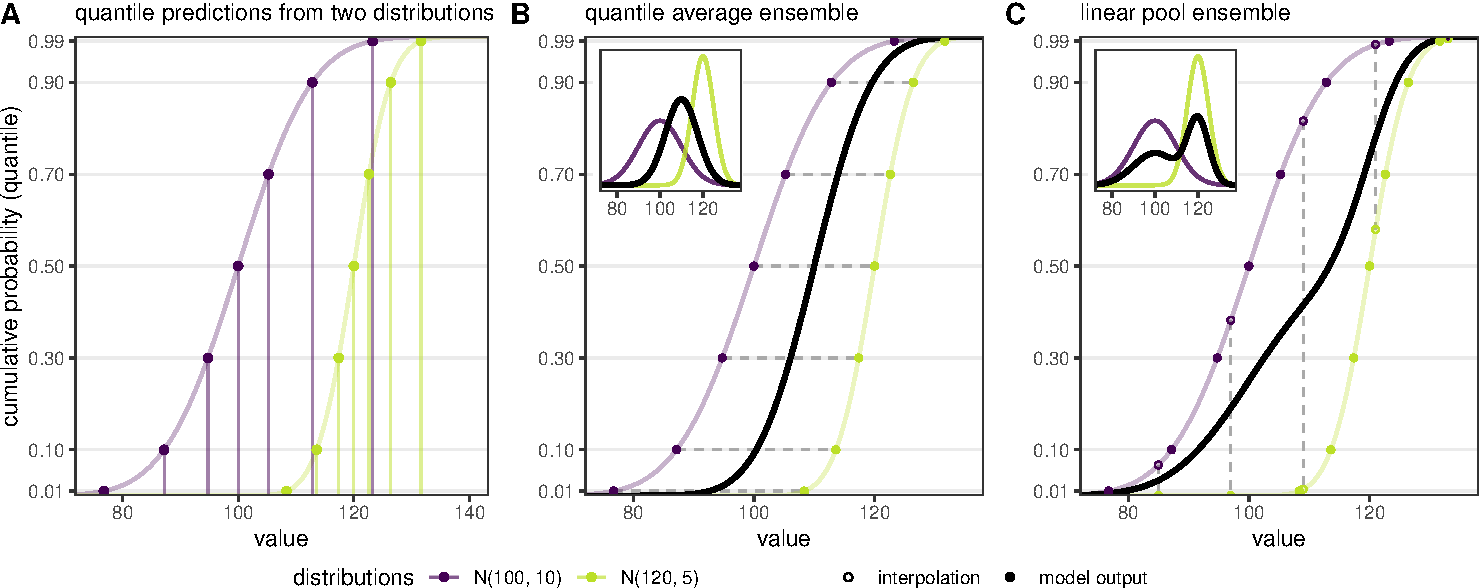
\includegraphics{hubEnsembles_manuscript_files/figure-pdf/fig-example-quantile-average-and-linear-pool-1.pdf}

}

\caption{\label{fig-example-quantile-average-and-linear-pool}(Panel A)
Example of quantile output type predictions. In this example, points
show model output collected for seven fixed quantile levels (\(\theta\)
= 0.01, 0.1, 0.3, 0.5, 0.7, 0.9, and 0.99) from two distributions
(\(N(100, 10)\) in purple and \(N(120, 5)\) in green), with the
underlying cumulative distribution functions (CDFs) shown with curves.
The y-axis ticks show each of the fixed quantile levels. The associated
values for each fixed quantile level do not align across distributions
(vertical lines). (Panel B) Quantile average ensemble, which is
calculated by averaging values for each fixed quantile level
(represented by horizontal dashed gray lines). The distributions and
corresponding model outputs from panel A are re-plotted and the black
line shows the resulting quantile average ensemble. Inset shows
corresponding probability density functions (PDFs). (Panel C) Linear
pool ensemble, which is calculated by averaging cumulative probabilities
for each fixed value (represented by vertical dashed gray lines). The
distributions and corresponding model outputs from panel A are
re-plotted. To calculate the linear pool in this case, where model
outputs are not defined for the same values, the model outputs are used
to interpolate the full CDF for each distribution from which quantiles
can be extracted for fixed values (shown with open circles). The black
line shows the resulting linear pool average ensemble. Inset shows
corresponding PDFs.}

\end{figure}%

Given that LOP cannot be directly calculated from quantile predictions,
we must first obtain an estimate of the CDF for each component
distribution from the provided quantiles, combine the CDFs, then
calculate the quantiles using the ensemble's CDF. We perform this
calculation in three main steps, assisted by the \pkg{distfromq} package
\citep{distfromq} for the first two:

\begin{enumerate}
\def\labelenumi{\arabic{enumi}.}
\tightlist
\item
  Interpolate and extrapolate from the provided quantiles for each
  component model to obtain an estimate of the CDF of that particular
  distribution.
\item
  Draw samples from each component model distribution. To reduce Monte
  Carlo variability, we use quasi-random samples corresponding to
  quantiles of the estimated distribution
  \citep{niederreiter1992quasirandom}.
\item
  Pool the samples from all component models and extract the desired
  quantiles.
\end{enumerate}

For step 1, functionality in the \pkg{distfromq} package uses a
monotonic cubic spline for interpolation on the interior of the provided
quantiles. The user may choose one of several distributions to perform
extrapolation of the CDF tails. These include normal, lognormal, and
cauchy distributions, with ``normal'' set as the default. A
location-scale parameterization is used, with separate location and
scale parameters chosen in the lower and upper tails so as to match the
two most extreme quantiles. The sampling process described in steps 2
and 3 approximates the linear pool calculation described in
Section~\ref{sec-defs}.

\section{Basic demonstration of functionality}\label{sec-simple-ex}

In this section, we provide a simple example to illustrate the two main
functions in \pkg{hubEnsembles}, \texttt{simple\_ensemble()} and
\texttt{linear\_pool()}.

\subsection{Example data: a forecast
hub}\label{example-data-a-forecast-hub}

\begin{longtable}[]{@{}
  >{\raggedright\arraybackslash}p{(\columnwidth - 10\tabcolsep) * \real{0.2169}}
  >{\raggedright\arraybackslash}p{(\columnwidth - 10\tabcolsep) * \real{0.1928}}
  >{\raggedleft\arraybackslash}p{(\columnwidth - 10\tabcolsep) * \real{0.1205}}
  >{\raggedright\arraybackslash}p{(\columnwidth - 10\tabcolsep) * \real{0.1687}}
  >{\raggedright\arraybackslash}p{(\columnwidth - 10\tabcolsep) * \real{0.2048}}
  >{\raggedleft\arraybackslash}p{(\columnwidth - 10\tabcolsep) * \real{0.0964}}@{}}

\toprule\noalign{}
\begin{minipage}[b]{\linewidth}\raggedright
\texttt{model\_id}
\end{minipage} & \begin{minipage}[b]{\linewidth}\raggedright
\texttt{target}
\end{minipage} & \begin{minipage}[b]{\linewidth}\raggedleft
\texttt{horizon}
\end{minipage} & \begin{minipage}[b]{\linewidth}\raggedright
\texttt{output\_type}
\end{minipage} & \begin{minipage}[b]{\linewidth}\raggedright
\texttt{output\_type\_id}
\end{minipage} & \begin{minipage}[b]{\linewidth}\raggedleft
\texttt{value}
\end{minipage} \\
\midrule\noalign{}
\endhead
\bottomrule\noalign{}
\endlastfoot
Flusight-baseline & wk inc flu hosp & 1 & quantile & 0.05 & 496 \\
Flusight-baseline & wk inc flu hosp & 1 & quantile & 0.25 & 566 \\
Flusight-baseline & wk inc flu hosp & 1 & quantile & 0.75 & 598 \\
Flusight-baseline & wk inc flu hosp & 1 & quantile & 0.95 & 668 \\
Flusight-baseline & wk inc flu hosp & 1 & median & NA & 582 \\
MOBS-GLEAM\_FLUH & wk inc flu hosp & 1 & quantile & 0.05 & 446 \\
MOBS-GLEAM\_FLUH & wk inc flu hosp & 1 & quantile & 0.25 & 563 \\
MOBS-GLEAM\_FLUH & wk inc flu hosp & 1 & quantile & 0.75 & 803 \\
MOBS-GLEAM\_FLUH & wk inc flu hosp & 1 & quantile & 0.95 & 1097 \\
MOBS-GLEAM\_FLUH & wk inc flu hosp & 1 & median & NA & 664 \\
PSI-DICE & wk inc flu hosp & 1 & quantile & 0.05 & 290 \\
PSI-DICE & wk inc flu hosp & 1 & quantile & 0.25 & 496 \\
PSI-DICE & wk inc flu hosp & 1 & quantile & 0.75 & 712 \\
PSI-DICE & wk inc flu hosp & 1 & quantile & 0.95 & 843 \\
PSI-DICE & wk inc flu hosp & 1 & median & NA & 613 \\


\caption{\label{tbl-example-model-outputs}Example model output for
forecasts of incident influenza hospitalizations. A subset of example
model output is shown: 1-week ahead quantile forecasts made on
2022-12-17 for Massachusetts from three distinct models; only the median
and 5th, 25th, 75th and 95th quantiles are displayed. The
\texttt{location}, \texttt{reference\_date} and
\texttt{target\_end\_date} columns have been omitted for brevity. This
example data is provided in the \pkg{hubExamples} package.}

\tabularnewline
\end{longtable}

We will use an example hub provided by the hubverse to demonstrate the
functionality of the \pkg{hubEnsembles} package \citep{hubverse_docs}.
This example hub was generated with forecasts from the FluSight
forecasting challenge, which will be discussed in detail in
Section~\ref{sec-case-study}. The example hub includes both example
model output data and target data (sometimes known as ``truth'' data),
which are included in the \pkg{hubExamples} package as data objects
named \texttt{forecast\_outputs} and \texttt{forecast\_target\_ts}. The
toy dataset of model output contains predictions for only a small subset
rows of select dates, locations, and output type IDs, far fewer than an
actual modeling hub would typically collect.

The model output data includes quantile, mean and median forecasts of
future incident influenza hospitalizations and PMF forecasts of
hospitalization intensity. Each forecast is made for five task ID
variables, including the location for which the forecast was made
(\texttt{location}), the date on which the forecast was made
(\texttt{reference\_date}), the number of steps ahead
(\texttt{horizon}), the date of the forecast prediction (a combination
of the date the forecast was made and the forecast horizon,
\texttt{target\_end\_date}), and the forecast target (\texttt{target}).
Table~\ref{tbl-example-model-outputs} provides an example set of
quantile forecasts included in this example model output. In
Table~\ref{tbl-example-model-outputs}, we show only the median, the
50\%, and 90\% prediction intervals, although other intervals and mean
forecasts are included in the example model output data.

We also have corresponding target data included in the \pkg{hubExamples}
package (Table~\ref{tbl-example-target-data}). The example target data
provide observed incident influenza hospitalizations
(\texttt{observation}) in a given week (\texttt{date}) and for a given
location (\texttt{location}). This target data could be used as
calibration data for generating forecasts or for evaluating the
forecasts post hoc. The forecast-specific task ID variables
\texttt{reference\_date} and \texttt{horizon} are not relevant for the
target data.

\begin{longtable}[]{@{}llr@{}}

\toprule\noalign{}
\texttt{date} & \texttt{location} & \texttt{observation} \\
\midrule\noalign{}
\endhead
\bottomrule\noalign{}
\endlastfoot
2022-11-05 & 25 & 31 \\
2022-11-12 & 25 & 43 \\
2022-11-19 & 25 & 79 \\
2022-11-26 & 25 & 221 \\
2022-12-03 & 25 & 446 \\
2022-12-10 & 25 & 578 \\
2022-12-17 & 25 & 694 \\
2022-12-24 & 25 & 769 \\
2022-12-31 & 25 & 733 \\
2023-01-07 & 25 & 466 \\
2023-01-14 & 25 & 238 \\
2023-01-21 & 25 & 122 \\
2023-01-28 & 25 & 71 \\


\caption{\label{tbl-example-target-data}Example target data for incident
influenza hospitalizations. This table includes target data from
2022-11-01 and 2023-02-01. This target data is provided in the
\pkg{hubExamples} package.}

\tabularnewline
\end{longtable}

We can plot these forecasts and the target data using the
\texttt{plot\_step\_ahead\_model\_output()} function from \pkg{hubVis},
another package for visualizing model outputs from the hubverse suite
(Figure~\ref{fig-plot-ex-mods}). We subset the model output data and the
target data to the location and time horizons we are interested in.

\begin{verbatim}
R> model_outputs_plot <- hubExamples::forecast_outputs |>
+    hubUtils::as_model_out_tbl() |>
+    dplyr::filter(
+      location == "25",
+      output_type %in% c("median", "mean", "quantile"),
+      reference_date == "2022-12-17"
+    )
R> target_data_plot <- hubExamples::forecast_target_ts |>
+    dplyr::filter(
+      location == "25",
+      date >= "2022-11-01", date <= "2023-02-01"
+    )
R> hubVis::plot_step_ahead_model_output(
+    model_output_data = model_outputs_plot,
+    target_data = target_data_plot,
+    facet = "model_id",
+    facet_nrow = 1,
+    interactive = FALSE,
+    intervals = c(0.5, 0.9),
+    show_legend = FALSE,
+    use_median_as_point = TRUE,
+    x_col_name = "target_end_date", 
+    x_target_col_name = "date"
+  ) +
+    theme_bw() +
+    labs(y = "incident hospitalizations")
\end{verbatim}

\begin{figure}[H]

\centering{

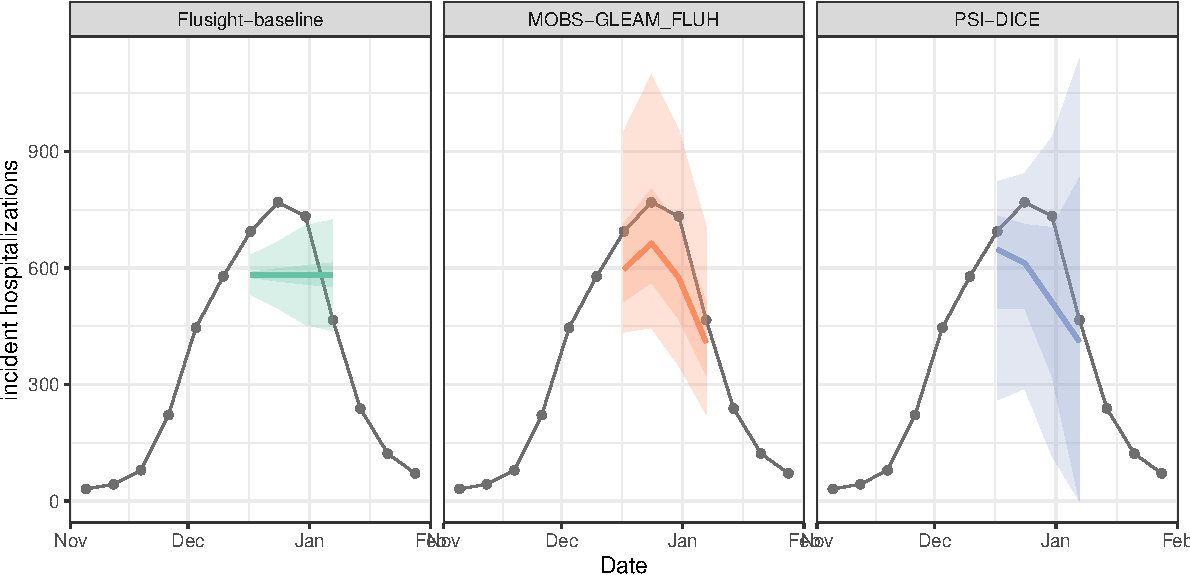
\includegraphics{hubEnsembles_manuscript_files/figure-pdf/fig-plot-ex-mods-1.pdf}

}

\caption{\label{fig-plot-ex-mods}One example set of quantile forecasts
of weekly incident influenza hospitalizations in Massachusetts from each
of three models (panels). Forecasts are represented by a median (line),
50\% and 90\% prediction intervals (ribbons). Gray points represent
observed incident hospitalizations.}

\end{figure}%

Next, we examine the PMF target in the example model output data. For
this target, teams forecasted the probability that hospitalization
intensity will be ``low'', ``moderate'', ``high'', or ``very high''.
These hospitalization intensity categories are determined by thresholds
for weekly hospital admissions per 100,000 population. In other words,
``low'' hospitalization intensity in a given week means few incident
influenza hospitalizations per 100,000 population are predicted, whereas
``very high'' hospitalization intensity means many hospitalizations per
100,000 population are predicted. These forecasts are made for the same
task ID variables as the \texttt{quantile} forecasts of incident
hospitalizations, other than the target, which is ``wk flu hosp rate
category'' for these categorical predictions.

\begin{longtable}[]{@{}
  >{\raggedright\arraybackslash}p{(\columnwidth - 10\tabcolsep) * \real{0.1935}}
  >{\raggedright\arraybackslash}p{(\columnwidth - 10\tabcolsep) * \real{0.2796}}
  >{\raggedleft\arraybackslash}p{(\columnwidth - 10\tabcolsep) * \real{0.1075}}
  >{\raggedright\arraybackslash}p{(\columnwidth - 10\tabcolsep) * \real{0.1505}}
  >{\raggedright\arraybackslash}p{(\columnwidth - 10\tabcolsep) * \real{0.1828}}
  >{\raggedleft\arraybackslash}p{(\columnwidth - 10\tabcolsep) * \real{0.0860}}@{}}

\toprule\noalign{}
\begin{minipage}[b]{\linewidth}\raggedright
\texttt{model\_id}
\end{minipage} & \begin{minipage}[b]{\linewidth}\raggedright
\texttt{target}
\end{minipage} & \begin{minipage}[b]{\linewidth}\raggedleft
\texttt{horizon}
\end{minipage} & \begin{minipage}[b]{\linewidth}\raggedright
\texttt{output\_type}
\end{minipage} & \begin{minipage}[b]{\linewidth}\raggedright
\texttt{output\_type\_id}
\end{minipage} & \begin{minipage}[b]{\linewidth}\raggedleft
\texttt{value}
\end{minipage} \\
\midrule\noalign{}
\endhead
\bottomrule\noalign{}
\endlastfoot
Flusight-baseline & wk flu hosp rate category & 1 & pmf & low & 0.00 \\
Flusight-baseline & wk flu hosp rate category & 1 & pmf & moderate &
0.00 \\
Flusight-baseline & wk flu hosp rate category & 1 & pmf & high & 0.07 \\
Flusight-baseline & wk flu hosp rate category & 1 & pmf & very high &
0.92 \\
MOBS-GLEAM\_FLUH & wk flu hosp rate category & 1 & pmf & low & 0.00 \\
MOBS-GLEAM\_FLUH & wk flu hosp rate category & 1 & pmf & moderate &
0.00 \\
MOBS-GLEAM\_FLUH & wk flu hosp rate category & 1 & pmf & high & 0.16 \\
MOBS-GLEAM\_FLUH & wk flu hosp rate category & 1 & pmf & very high &
0.83 \\
PSI-DICE & wk flu hosp rate category & 1 & pmf & low & 0.01 \\
PSI-DICE & wk flu hosp rate category & 1 & pmf & moderate & 0.07 \\
PSI-DICE & wk flu hosp rate category & 1 & pmf & high & 0.22 \\
PSI-DICE & wk flu hosp rate category & 1 & pmf & very high & 0.70 \\


\caption{\label{tbl-example-forecasts-pmf}Example PMF model output for
forecasts of incident influenza hospitalization intensity. A subset of
example model output is shown: 1-week ahead PMF forecasts made on
2022-12-17 for Massachusetts from three distinct models. We round the
forecasted probability (in the \texttt{value} column) to two digits. The
\texttt{location}, \texttt{reference\_date} and
\texttt{target\_end\_date} columns have been omitted for brevity. This
example data is provided in the \pkg{hubExamples} package.}

\tabularnewline
\end{longtable}

We show a representative example of the hospitalization intensity
category forecasts in Table~\ref{tbl-example-forecasts-pmf}. Because
these forecasts are PMF output type, the \texttt{output\_type\_id}
column specifies the bin of hospitalization intensity and the
\texttt{value} column provides the forecasted probability of
hospitalization incidence being in that category. Values sum to 1 across
bins. For the MOBS-GLEAM\_FLUH and PSI-DICE models, incidence is
forecasted to decrease over the horizon (Figure~\ref{fig-plot-ex-mods}),
and correspondingly, there is lower probability of ``high'' and ``very
high'' hospitalization intensity for later horizons
(Figure~\ref{fig-plot-ex-mods-pmf}).

\begin{figure}

\centering{

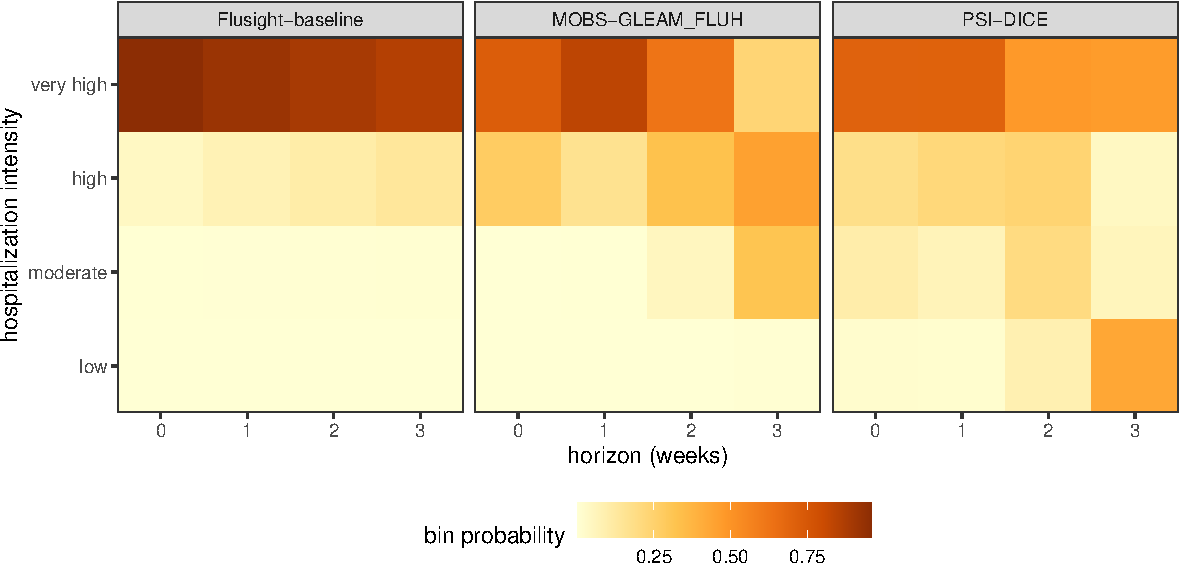
\includegraphics{hubEnsembles_manuscript_files/figure-pdf/fig-plot-ex-mods-pmf-1.pdf}

}

\caption{\label{fig-plot-ex-mods-pmf}One example PMF forecast of
incident influenza hospitalization intensity is shown for each of three
models (panels). Each cell shows the forecasted probability of a given
hospitalization intensity bin (low, moderate, high, and very high) for
each forecast horizon (0-3 weeks ahead). Darker colors indicate higher
forecasted probability.}

\end{figure}%

\subsection{Creating ensembles with
simple\_ensemble}\label{creating-ensembles-with-simple_ensemble}

Using the default options for \texttt{simple\_ensemble()}, we can
generate an equally weighted mean ensemble for each unique combination
of values for the task ID variables, the \texttt{output\_type} and the
\texttt{output\_type\_id}. Recall that this means different ensemble
methods will be used for different output types: for the
\texttt{quantile} output type in our example data, the resulting
ensemble is a quantile average, while for the PMF output type, the
ensemble is a linear pool.

\begin{verbatim}
R> mean_ens <- hubEnsembles::simple_ensemble(
+    hubExamples::forecast_outputs,
+    model_id = "simple-ensemble-mean"
+  )
\end{verbatim}

The resulting model output has the same structure as the original model
output data (Table~\ref{tbl-mean-ensemble}), with columns for model ID,
task ID variables, output type, output type ID, and value. We also use
\texttt{model\_id\ =\ "simple-ensemble-mean"} to change the name of this
ensemble in the resulting model output; if not specified, the default
will be ``hub-ensemble''.

\begin{longtable}[]{@{}
  >{\raggedright\arraybackslash}p{(\columnwidth - 10\tabcolsep) * \real{0.2188}}
  >{\raggedright\arraybackslash}p{(\columnwidth - 10\tabcolsep) * \real{0.2708}}
  >{\raggedleft\arraybackslash}p{(\columnwidth - 10\tabcolsep) * \real{0.1042}}
  >{\raggedright\arraybackslash}p{(\columnwidth - 10\tabcolsep) * \real{0.1458}}
  >{\raggedright\arraybackslash}p{(\columnwidth - 10\tabcolsep) * \real{0.1771}}
  >{\raggedleft\arraybackslash}p{(\columnwidth - 10\tabcolsep) * \real{0.0833}}@{}}

\toprule\noalign{}
\begin{minipage}[b]{\linewidth}\raggedright
\texttt{model\_id}
\end{minipage} & \begin{minipage}[b]{\linewidth}\raggedright
\texttt{target}
\end{minipage} & \begin{minipage}[b]{\linewidth}\raggedleft
\texttt{horizon}
\end{minipage} & \begin{minipage}[b]{\linewidth}\raggedright
\texttt{output\_type}
\end{minipage} & \begin{minipage}[b]{\linewidth}\raggedright
\texttt{output\_type\_id}
\end{minipage} & \begin{minipage}[b]{\linewidth}\raggedleft
\texttt{value}
\end{minipage} \\
\midrule\noalign{}
\endhead
\bottomrule\noalign{}
\endlastfoot
simple-ensemble-mean & wk flu hosp rate category & 1 & pmf & high &
0.15 \\
simple-ensemble-mean & wk flu hosp rate category & 1 & pmf & low &
0.00 \\
simple-ensemble-mean & wk flu hosp rate category & 1 & pmf & moderate &
0.02 \\
simple-ensemble-mean & wk flu hosp rate category & 1 & pmf & very high &
0.82 \\
simple-ensemble-mean & wk inc flu hosp & 1 & median & NA & 619.67 \\
simple-ensemble-mean & wk inc flu hosp & 1 & quantile & 0.25 & 541.67 \\
simple-ensemble-mean & wk inc flu hosp & 1 & quantile & 0.75 & 704.33 \\


\caption{\label{tbl-mean-ensemble}Mean ensemble model output. The values
in the \texttt{model\_id} column are determined by the argument
\texttt{simple\_ensemble(...,\ model\_id\ =\ )}. A subset of ensemble
model output is shown: 1-week ahead PMF forecasts made on 2022-12-17 for
Massachusetts. Results are generated for all output types. Here, we show
only the median, 25th and 75th quantiles for the quantile output type
and all bins for the PMF output type. The \texttt{location},
\texttt{reference\_date} and \texttt{target\_end\_date} columns have
been omitted for brevity, and the \texttt{value} column is rounded to
two digits.}

\tabularnewline
\end{longtable}

\subsubsection{Changing the aggregation
function}\label{changing-the-aggregation-function}

We can change the function that is used to aggregate model outputs. For
example, we may want to calculate a median of the component models'
submitted values for each quantile. We do so by specifying
\texttt{agg\_fun\ =\ median}.

\begin{verbatim}
R> median_ens <- hubExamples::forecast_outputs |>
+  hubEnsembles::simple_ensemble(
+    agg_fun = median,
+    model_id = "simple-ensemble-median"
+  )
\end{verbatim}

Custom functions can also be passed into the \texttt{agg\_fun} argument.
We illustrate this by defining a custom function to compute the ensemble
prediction as a geometric mean of the component model predictions. Any
custom function to be used must have an argument \texttt{x} for the
vector of numeric values to summarize, and if relevant, an argument
\texttt{w} of numeric weights.

\begin{verbatim}
R> geometric_mean <- function(x) {
+    n <- length(x)
+    return(prod(x)^(1 / n))
+  }
R> geometric_mean_ens <- hubExamples::forecast_outputs |>
+    hubEnsembles::simple_ensemble(
+      agg_fun = geometric_mean,
+      model_id = "simple-ensemble-geometric"
+    )
\end{verbatim}

As expected, the mean, median, and geometric mean each give us slightly
different resulting ensembles. The median point estimates, 50\%
prediction intervals, and 90\% prediction intervals in
Figure~\ref{fig-plot-ensembles} demonstrate this.

\begin{figure}

\centering{

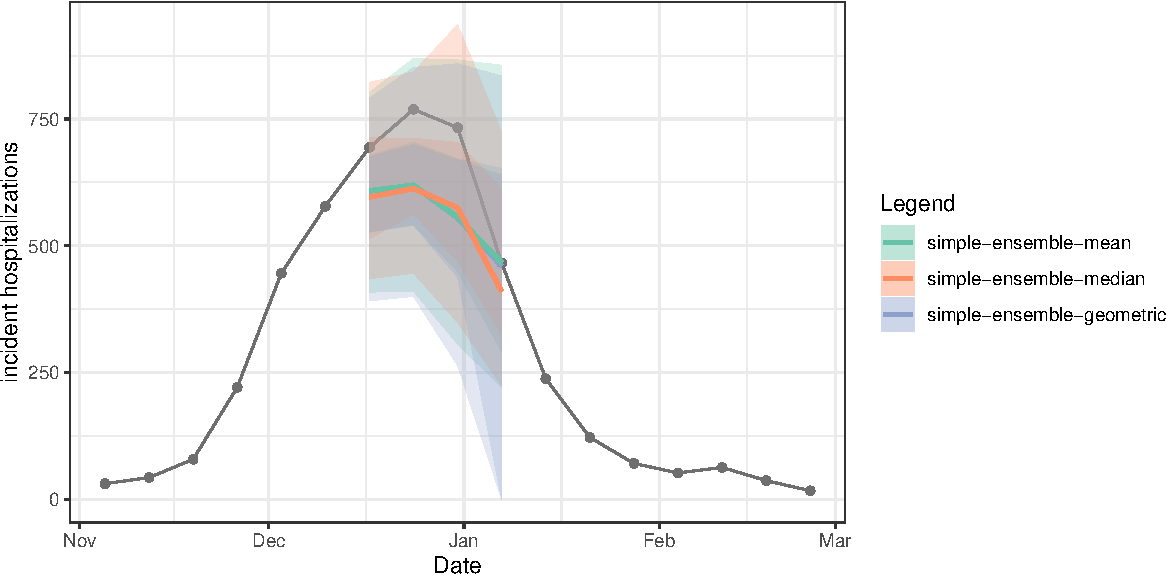
\includegraphics{hubEnsembles_manuscript_files/figure-pdf/fig-plot-ensembles-1.pdf}

}

\caption{\label{fig-plot-ensembles}Three different ensembles for weekly
incident influenza hospitalizations in Massachusetts. Each ensemble
combines individual predictions from the example hub
(Figure~\ref{fig-plot-ex-mods}) using a different method: arithmetic
mean, geometric mean, or median. All methods correspond to variations of
the quantile average approach. Ensembles are represented by a median
(line), 50\% and 90\% prediction intervals (ribbons). Geometric mean
ensemble and simple mean ensemble generate similar estimates in this
case.}

\end{figure}%

\subsubsection{Weighting model
contributions}\label{weighting-model-contributions}

We can weight the contributions of each model in the ensemble using the
\texttt{weights} argument of \texttt{simple\_ensemble()}. This argument
takes a \texttt{data.frame} that should include a \texttt{model\_id}
column containing each unique model ID and a \texttt{weight} column. In
the following example, we include the baseline model in the ensemble,
but give it less weight than the other forecasts.

\begin{verbatim}
R> model_weights <- data.frame(
+    model_id = c("MOBS-GLEAM_FLUH", "PSI-DICE", "simple_hub-baseline"),
+    weight = c(0.4, 0.4, 0.2)
+  )
R> weighted_mean_ens <- hubExamples::forecast_outputs |>
+    hubEnsembles::simple_ensemble(
+      weights = model_weights,
+      model_id = "simple-ensemble-weighted-mean"
+    )
\end{verbatim}

\subsection{Creating ensembles with
linear\_pool}\label{creating-ensembles-with-linear_pool}

We can also generate a linear pool ensemble, or distributional mixture,
using the \texttt{linear\_pool()} function; this function can be applied
to predictions with an \texttt{output\_type} of mean, quantile, CDF, or
PMF. Our example hub includes median output type, so we exclude it from
the calculation.

\begin{verbatim}
R> linear_pool_ens <- hubExamples::forecast_outputs |>
+    dplyr::filter(output_type != "median") |>
+    hubEnsembles::linear_pool(model_id = "linear-pool")
\end{verbatim}

As described above, for \texttt{quantile} model outputs, the
\texttt{linear\_pool} function approximates the full probability
distribution for each component prediction using the value-quantile
pairs provided by that model, and then obtains quasi-random samples from
that distributional estimate. The number of samples drawn from the
distribution of each component model defaults to \texttt{1e4}, but this
can be changed using the \texttt{n\_samples} argument.

In Figure~\ref{fig-plot-ex-quantile-and-linear-pool}, we compare
ensemble results generated by \texttt{simple\_ensemble()} and
\texttt{linear\_pool()} for model outputs of output types PMF and
quantile. As expected, the results from the two functions are equivalent
for the PMF output type: for this output type, the
\texttt{simple\_ensemble()} method averages the predicted probability of
each category across the component models, which is the definition of
the linear pool ensemble method. This is not the case for the quantile
output type, because the \texttt{simple\_ensemble()} is computing a
quantile average.

\begin{figure}

\centering{

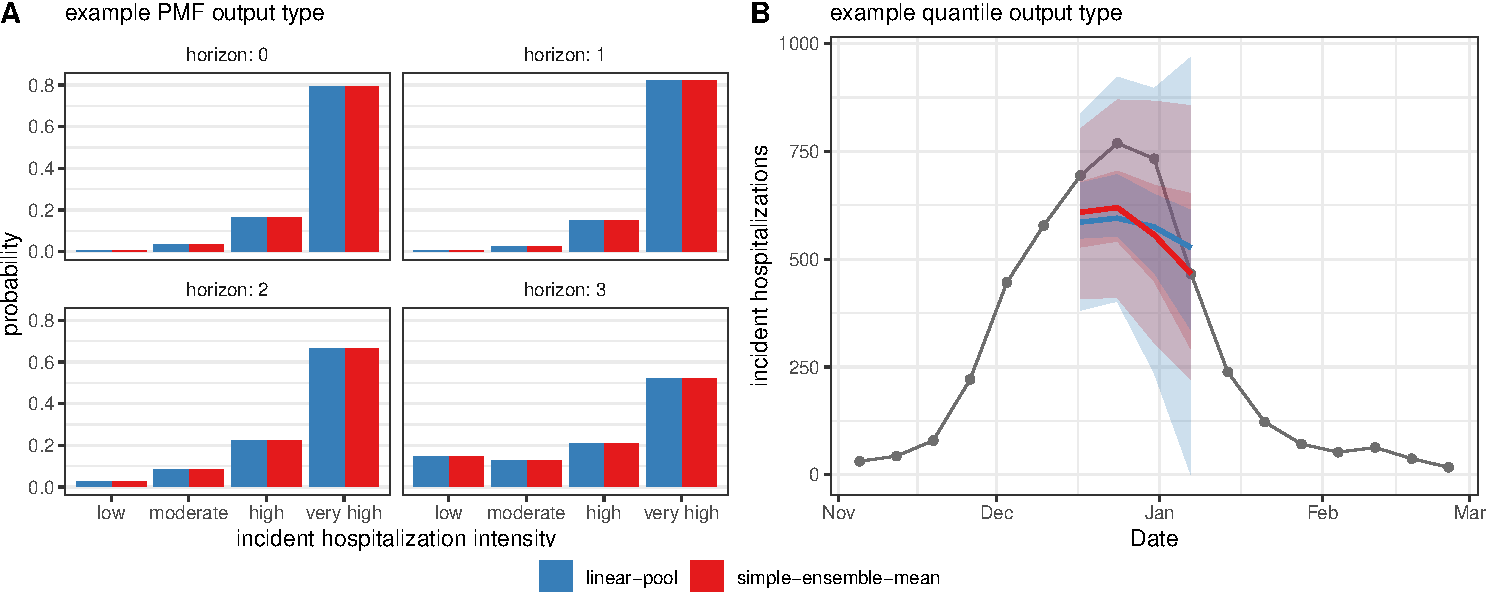
\includegraphics{hubEnsembles_manuscript_files/figure-pdf/fig-plot-ex-quantile-and-linear-pool-1.pdf}

}

\caption{\label{fig-plot-ex-quantile-and-linear-pool}Comparison of
results from \texttt{linear\_pool()} (blue) and
\texttt{simple\_ensemble()} (red) . (Panel A) Ensemble predictions of
Massachusetts incident influenza hospitalization intensity (classified
as low, moderate, high, or very high), which provide an example of PMF
output type. (Panel B) Ensemble predictions of weekly incident influenza
hospitalizations in Massachusetts, which provide an example of quantile
output type. Note, for quantile output type, \texttt{simple\_ensemble()}
corresponds to a quantile average. Ensembles combine individual models
from the example hub, and are represented by a median (line), 50\% and
90\% prediction intervals (ribbons) (Figure~\ref{fig-plot-ex-mods}).}

\end{figure}%

\section{Example: in-depth analysis of forecast
data}\label{sec-case-study}

To further demonstrate the utility of the \pkg{hubEnsembles} package and
the differences between the two ensembling functions, we examine a more
complex example. Unlike the previous section's basic showcase of
functionality, we use this case study to provide a more complete
analysis that compares and evaluates ensemble model performance using
real forecasts collected by a modeling hub, with an overarching goal of
choosing a single best ensembling approach for the application.

Since 2013, the US Centers for Disease Control and Prevention (CDC) has
been soliciting forecasts of seasonal influenza from modeling teams
through a collaborative challenge called FluSight \citep{cdc_flusight}.
We use a subset of these predictions to create four equally-weighted
ensembles with \texttt{simple\_ensemble()} and \texttt{linear\_pool()}
and compare the resulting ensembles' performance. The ensembling methods
chosen for this case study consist of a quantile (arithmetic) mean, a
quantile median, a linear pool with normal tails, and a linear pool with
lognormal tails. Note that only a select portion of the code is shown in
this manuscript for brevity, although all the functions and scripts used
to generate the case study results can be found in the associated GitHub
repository
(\url{https://github.com/Infectious-Disease-Modeling-Hubs/hubEnsemblesManuscript}).
More specifically, the figures and tables supporting this analysis are
generated reproducibly using data from rds files stored in the
\texttt{analysis/data/raw-data} directory and scripts in the
\texttt{inst} directory of the repository.

\subsection{Data and Methods}\label{data-and-methods}

We begin by querying the component forecasts used to generate the four
ensembles from Zoltar \citep{reich_zoltar_2021}, a repository designed
to archive forecasts created by the Reich Lab at UMass Amherst. For this
analysis we only consider FluSight predictions in a quantile format from
the 2021-2022 and 2022-2023 seasons. These forecasts were stored in two
data objects, split by season, called
\texttt{flu\_forecasts-raw\_21-22.rds} and
\texttt{flu\_forecasts-raw\_22-23.rds}, and a subset of the the second
is shown below in Table~\ref{tbl-raw-flu-forecasts}.

\begin{verbatim}
R> flu_forecasts_raw_21_22 <- readr::read_rds(
+    here::here("analysis/data/raw_data/flu_forecasts-zoltar_21-22.rds")
+  )
R> flu_forecasts_raw_22_23 <- readr::read_rds(
+    here::here("analysis/data/raw_data/flu_forecasts-zoltar_22-23.rds")
+  )
R> flu_forecasts_raw <- rbind(flu_forecasts_raw_21_22, flu_forecasts_raw_22_23)
\end{verbatim}

\begin{longtable}[]{@{}
  >{\raggedright\arraybackslash}p{(\columnwidth - 16\tabcolsep) * \real{0.2095}}
  >{\raggedright\arraybackslash}p{(\columnwidth - 16\tabcolsep) * \real{0.2286}}
  >{\raggedright\arraybackslash}p{(\columnwidth - 16\tabcolsep) * \real{0.0857}}
  >{\raggedleft\arraybackslash}p{(\columnwidth - 16\tabcolsep) * \real{0.0762}}
  >{\raggedright\arraybackslash}p{(\columnwidth - 16\tabcolsep) * \real{0.0571}}
  >{\raggedright\arraybackslash}p{(\columnwidth - 16\tabcolsep) * \real{0.0667}}
  >{\raggedright\arraybackslash}p{(\columnwidth - 16\tabcolsep) * \real{0.0857}}
  >{\raggedleft\arraybackslash}p{(\columnwidth - 16\tabcolsep) * \real{0.1048}}
  >{\raggedright\arraybackslash}p{(\columnwidth - 16\tabcolsep) * \real{0.0857}}@{}}

\toprule\noalign{}
\begin{minipage}[b]{\linewidth}\raggedright
\texttt{model}
\end{minipage} & \begin{minipage}[b]{\linewidth}\raggedright
\texttt{target}
\end{minipage} & \begin{minipage}[b]{\linewidth}\raggedright
\texttt{class}
\end{minipage} & \begin{minipage}[b]{\linewidth}\raggedleft
\texttt{value}
\end{minipage} & \begin{minipage}[b]{\linewidth}\raggedright
\texttt{cat}
\end{minipage} & \begin{minipage}[b]{\linewidth}\raggedright
\texttt{prob}
\end{minipage} & \begin{minipage}[b]{\linewidth}\raggedright
\texttt{sample}
\end{minipage} & \begin{minipage}[b]{\linewidth}\raggedleft
\texttt{quantile}
\end{minipage} & \begin{minipage}[b]{\linewidth}\raggedright
\texttt{family}
\end{minipage} \\
\midrule\noalign{}
\endhead
\bottomrule\noalign{}
\endlastfoot
UMass-trends\_ensemble & 1 wk ahead inc flu hosp & quantile & 12 & NA &
NA & NA & 0.025 & NA \\
UMass-trends\_ensemble & 1 wk ahead inc flu hosp & quantile & 17 & NA &
NA & NA & 0.100 & NA \\
UMass-trends\_ensemble & 1 wk ahead inc flu hosp & quantile & 25 & NA &
NA & NA & 0.250 & NA \\
UMass-trends\_ensemble & 1 wk ahead inc flu hosp & quantile & 46 & NA &
NA & NA & 0.750 & NA \\
UMass-trends\_ensemble & 1 wk ahead inc flu hosp & quantile & 56 & NA &
NA & NA & 0.900 & NA \\
UMass-trends\_ensemble & 1 wk ahead inc flu hosp & quantile & 68 & NA &
NA & NA & 0.975 & NA \\


\caption{\label{tbl-raw-flu-forecasts}An example prediction of weekly
incident influenza hospitalizations pulled directly from Zoltar. The
example forecasts were made on May 15, 2023 for California at the 1 week
ahead horizon. The forecast was generated during the FluSight
forecasting challenge, then formatted according to Zoltar standards for
storage. The \texttt{timezero}, \texttt{season}, \texttt{unit},
\texttt{param1}, \texttt{param2}, and \texttt{param3} columns have been
omitted for brevity. (The \texttt{season} column has a value of
`2021-2022' or `2022-2023' while the last three `param' columns always
have a value of NA.)}

\tabularnewline
\end{longtable}

Forecasts must conform to hubverse standards to be fed into either of
the ensembling functions, so we first transform the raw forecasts using
the \texttt{as\_model\_out\_tbl()}\footnote{https://infectious-disease-modeling-hubs.github.io/hubUtils/reference/as\_model\_out\_tbl.html}
function from the \pkg{hubUtils} package. Here, we specify the task ID
variables \texttt{forecast\_date} (when the forecast was made),
\texttt{location}, \texttt{horizon}, and \texttt{target}.

\begin{verbatim}
R> flu_forecasts_hubverse <- flu_forecasts_raw |>
+    dplyr::rename(forecast_date = timezero, location=unit) |>
+    tidyr::separate(target, sep = " ", convert = TRUE,
+                    into = c("horizon", "target"), extra = "merge") |>
+    dplyr::mutate(target_end_date = 
+                    ceiling_date(forecast_date + weeks(horizon), "weeks") -
+                      days(1)) |>
+    as_model_out_tbl(
+      model_id_col = "model",
+      output_type_col = "class",
+      output_type_id_col = "quantile",
+      value_col = "value",
+      sep = "-",
+      trim_to_task_ids = FALSE,
+      hub_con = NULL,
+      task_id_cols = 
+        c("forecast_date", "location", "horizon", "target", target_end_date),
+      remove_empty = TRUE
+    )
\end{verbatim}

We filter out any predictions (defined by a unique combination of task
ID variables) that did not include all 23 quantiles specified by
FluSight
(\(\theta \in \{.010, 0.025, .050, .100, ..., .900, .950, .990\}\)). The
FluSight baseline and median ensemble models generated by the FluSight
hub are also excluded from the component forecasts. We chose to remove
the baseline from the ensemble calculations to match the composition of
models used to create FluSight-median.

With these inclusion criteria, the final data set of component forecasts
consists of predictions from 25 modeling teams and 42 distinct models,
53 forecast dates (one per week), 54 US locations, 4 horizons, 1 target,
and 23 quantiles. In the 2021-2022 season, 25 models made predictions
for 22 weeks spanning from late January 2022 to late June 2022, and in
the 2022-2023 season, there were 31 models making predictions for 31
weeks spanning mid-October 2022 to mid-May 2023. Fourteen of the 42
total models made forecasts for both seasons.

In both seasons, forecasts were made for the same locations (the 50 US
states, Washington DC, Puerto Rico, the Virgin Islands, and the US as a
whole), horizons (1 to 4 weeks ahead), quantiles (the 23 described
above), and target (week ahead incident flu hospitalization). The values
for the forecasts are always non-negative. In
Table~\ref{tbl-case-study-flu-forecasts}, we provide an example of these
predictions, showing select quantiles from a single model, forecast
date, horizon, and location.

\begin{longtable}[]{@{}
  >{\raggedright\arraybackslash}p{(\columnwidth - 10\tabcolsep) * \real{0.2366}}
  >{\raggedright\arraybackslash}p{(\columnwidth - 10\tabcolsep) * \real{0.2366}}
  >{\raggedleft\arraybackslash}p{(\columnwidth - 10\tabcolsep) * \real{0.1075}}
  >{\raggedright\arraybackslash}p{(\columnwidth - 10\tabcolsep) * \real{0.1505}}
  >{\raggedleft\arraybackslash}p{(\columnwidth - 10\tabcolsep) * \real{0.1828}}
  >{\raggedleft\arraybackslash}p{(\columnwidth - 10\tabcolsep) * \real{0.0860}}@{}}

\toprule\noalign{}
\begin{minipage}[b]{\linewidth}\raggedright
\texttt{model\_id}
\end{minipage} & \begin{minipage}[b]{\linewidth}\raggedright
\texttt{target}
\end{minipage} & \begin{minipage}[b]{\linewidth}\raggedleft
\texttt{horizon}
\end{minipage} & \begin{minipage}[b]{\linewidth}\raggedright
\texttt{output\_type}
\end{minipage} & \begin{minipage}[b]{\linewidth}\raggedleft
\texttt{output\_type\_id}
\end{minipage} & \begin{minipage}[b]{\linewidth}\raggedleft
\texttt{value}
\end{minipage} \\
\midrule\noalign{}
\endhead
\bottomrule\noalign{}
\endlastfoot
UMass-trends\_ensemble & wk ahead inc flu hosp & 1 & quantile & 0.025 &
12 \\
UMass-trends\_ensemble & wk ahead inc flu hosp & 1 & quantile & 0.100 &
17 \\
UMass-trends\_ensemble & wk ahead inc flu hosp & 1 & quantile & 0.250 &
25 \\
UMass-trends\_ensemble & wk ahead inc flu hosp & 1 & quantile & 0.750 &
46 \\
UMass-trends\_ensemble & wk ahead inc flu hosp & 1 & quantile & 0.900 &
56 \\
UMass-trends\_ensemble & wk ahead inc flu hosp & 1 & quantile & 0.975 &
68 \\


\caption{\label{tbl-case-study-flu-forecasts}An example prediction of
weekly incident influenza hospitalizations. The example model output was
made on May 15, 2023 for California at the 1 week ahead horizon. The
forecast was generated during the FluSight forecasting challenge, then
formatted according to hubverse standards post hoc. The
\texttt{location}, \texttt{forecast\_date}, and \texttt{season} columns
have been omitted for brevity; quantiles representing the endpoints of
the central 50\%, 80\% and 95\% prediction intervals are shown.}

\tabularnewline
\end{longtable}

Next, we combine the component model outputs to generate predictions
from each ensemble model. We begin by excluding the baseline model from
the set of predictions that will be combined. Then, we create one object
to store the ensemble results generated from each method we are
interested in comparing.

\begin{verbatim}
R> flu_forecasts_component <- dplyr::filter(
+    flu_forecasts_hubverse,
+    !model_id %in% c("Flusight-baseline", "Flusight-ensemble")
+  )
R> 
R> mean_ensemble <- flu_forecasts_component |>
+    hubEnsembles::simple_ensemble(
+      weights = NULL,
+      agg_fun = mean,
+      model_id = "mean-ensemble"
+    )
R> median_ensemble <- flu_forecasts_component |>
+    hubEnsembles::simple_ensemble(
+      weights = NULL,
+      agg_fun = median,
+      model_id = "median-ensemble"
+    )
R> lp_normal <- flu_forecasts_component |>
+    hubEnsembles::linear_pool(
+      weights = NULL,
+      n_samples = 1e5,
+      model_id = "lp-normal",
+      tail_dist = "norm"
+    )
R> lp_lognormal <- flu_forecasts_component |>
+    hubEnsembles::linear_pool(
+      weights = NULL,
+      n_samples = 1e5,
+      model_id = "lp-lognormal",
+      tail_dist = "lnorm"
+    ) 
\end{verbatim}

We evaluate the performance of these ensembles using scoring metrics
that measure the accuracy and calibration of their forecasts. Here, we
choose several common metrics in forecast evaluation, including mean
absolute error (MAE), weighted interval score (WIS)
\citep{bracher_evaluating_2021}, 50\% prediction interval (PI) coverage,
and 95\% PI coverage. MAE measures the average absolute error of a set
of point forecasts; smaller values of MAE indicate better forecast
accuracy. WIS is a generalization of MAE for probabilistic forecasts and
is an alternative to other common proper scoring rules which cannot be
evaluated directly for quantile forecasts
\citep{bracher_evaluating_2021}. WIS is made up of three component
penalties: (1) for over-prediction, (2) for under-prediction, and (3)
for the spread of each interval (where an interval is defined by a
symmetric set of two quantiles). This metric weights these penalties
across all prediction intervals provided. A lower WIS value indicates a
more accurate forecast \citep{bracher_evaluating_2021}. PI coverage
provides information about whether a forecast has accurately
characterized its uncertainty about future observations. The \(50\)\% PI
coverage rate measures the proportion of the time that 50\% prediction
intervals at that nominal level included the observed value; the 95\% PI
coverage rate is defined similarly. Achieving approximately nominal
(50\% or 95\%) coverage indicates a well-calibrated forecast.

We also use relative versions of WIS and MAE (rWIS and rMAE,
respectively) to understand how the ensemble performance compares to
that of the FluSight baseline model. These metrics are calculated as
\[\textrm{rWIS} = \frac{\textrm{WIS}_{\textrm{model }m}}{\textrm{WIS}_{\textrm{baseline}}} \hspace{3cm} \textrm{rMAE} = \frac{\textrm{MAE}_{\textrm{model }m}}{\textrm{MAE}_{\textrm{baseline}}},\]
where model \(m\) is any given model being compared against the
baseline. For both of these metrics, a value less than one indicates
better performance compared to the baseline while a value greater than
one indicates worse performance. By definition, the FluSight baseline
itself will always have a value of one for both of these metrics.

Each unique prediction from an ensemble model is scored against target
data using the \texttt{score\_forecasts()}\footnote{https://reichlab.io/covidHubUtils/reference/score\_forecasts.html}
function from the \pkg{covidHubUtils} package, as a hubverse package for
scoring and evaluation has not yet been fully implemented. This function
outputs each of the metrics described above. We use median forecasts
taken from the 0.5 quantile for the MAE evaluation.

\subsection{Performance results across
ensembles}\label{performance-results-across-ensembles}

The quantile median ensemble has the best overall performance in terms
of WIS and MAE (and the relative versions of these metrics), and has
coverage rates that were close to the nominal levels
(Table~\ref{tbl-overall-evaluation}). The two linear opinion pools has
very similar performance to each other. These methods have the
second-best performance as measured by WIS and MAE, but they have the
highest 50\% and 95\% coverage rates, with empirical coverage that was
well above the nominal coverage rate. The quantile mean performs the
worst of the ensembles with the highest MAE, which is substantially
different from that of the other ensembles.

\begin{longtable}[]{@{}
  >{\raggedright\arraybackslash}p{(\columnwidth - 12\tabcolsep) * \real{0.2469}}
  >{\raggedright\arraybackslash}p{(\columnwidth - 12\tabcolsep) * \real{0.1358}}
  >{\raggedright\arraybackslash}p{(\columnwidth - 12\tabcolsep) * \real{0.1235}}
  >{\raggedright\arraybackslash}p{(\columnwidth - 12\tabcolsep) * \real{0.1235}}
  >{\raggedright\arraybackslash}p{(\columnwidth - 12\tabcolsep) * \real{0.1235}}
  >{\raggedright\arraybackslash}p{(\columnwidth - 12\tabcolsep) * \real{0.1235}}
  >{\raggedright\arraybackslash}p{(\columnwidth - 12\tabcolsep) * \real{0.1235}}@{}}

\toprule\noalign{}
\begin{minipage}[b]{\linewidth}\raggedright
\texttt{model}
\end{minipage} & \begin{minipage}[b]{\linewidth}\raggedright
\texttt{wis}
\end{minipage} & \begin{minipage}[b]{\linewidth}\raggedright
\texttt{rwis}
\end{minipage} & \begin{minipage}[b]{\linewidth}\raggedright
\texttt{mae}
\end{minipage} & \begin{minipage}[b]{\linewidth}\raggedright
\texttt{rmae}
\end{minipage} & \begin{minipage}[b]{\linewidth}\raggedright
\texttt{cov50}
\end{minipage} & \begin{minipage}[b]{\linewidth}\raggedright
\texttt{cov95}
\end{minipage} \\
\midrule\noalign{}
\endhead
\bottomrule\noalign{}
\endlastfoot
\textbf{median-ensemble} & \textbf{18.158} & \textbf{0.794} &
\textbf{27.36} & \textbf{0.933} & 0.597 & \textbf{0.922} \\
lp-normal & 19.745 & 0.863 & 27.932 & 0.953 & 0.709 & 0.99 \\
lp-lognormal & 19.747 & 0.863 & 27.933 & 0.953 & 0.708 & 0.99 \\
mean-ensemble & 20.18 & 0.882 & 29.582 & 1.009 & \textbf{0.595} &
0.889 \\
Flusight-baseline & 22.876 & 1 & 29.315 & 1 & 0.604 & 0.881 \\


\caption{\label{tbl-overall-evaluation}Summary of overall model
performance across both seasons, averaged over all locations except the
US national location. The best value for each metric is bolded, though
the metric values are often quite similar among the models.}

\tabularnewline
\end{longtable}

Plots of the models' forecasts can aid our understanding about the
origin of these accuracy differences. For example, the linear opinion
pools consistently has some of the widest prediction intervals, and
consequently the highest coverage rates. The median ensemble, which has
the best WIS, balanced interval width with calibration best overall,
with narrower intervals than the linear pools that still achieved
near-nominal coverage on average across all time points. The quantile
mean's interval widths varies, though it usually has narrower intervals
than the linear pools. However, this model's point forecasts has a
larger error margin compared to the other ensembles, especially at
longer horizons. This pattern is demonstrated in
Figure~\ref{fig-plot-forecasts-hubVis} for the 4-week ahead forecast in
California following the 2022-23 season peak on December 5, 2022. Here
the quantile mean predicted a continued increase in hospitalizations, at
a steeper slope than the other ensemble methods.

\begin{figure}

\centering{

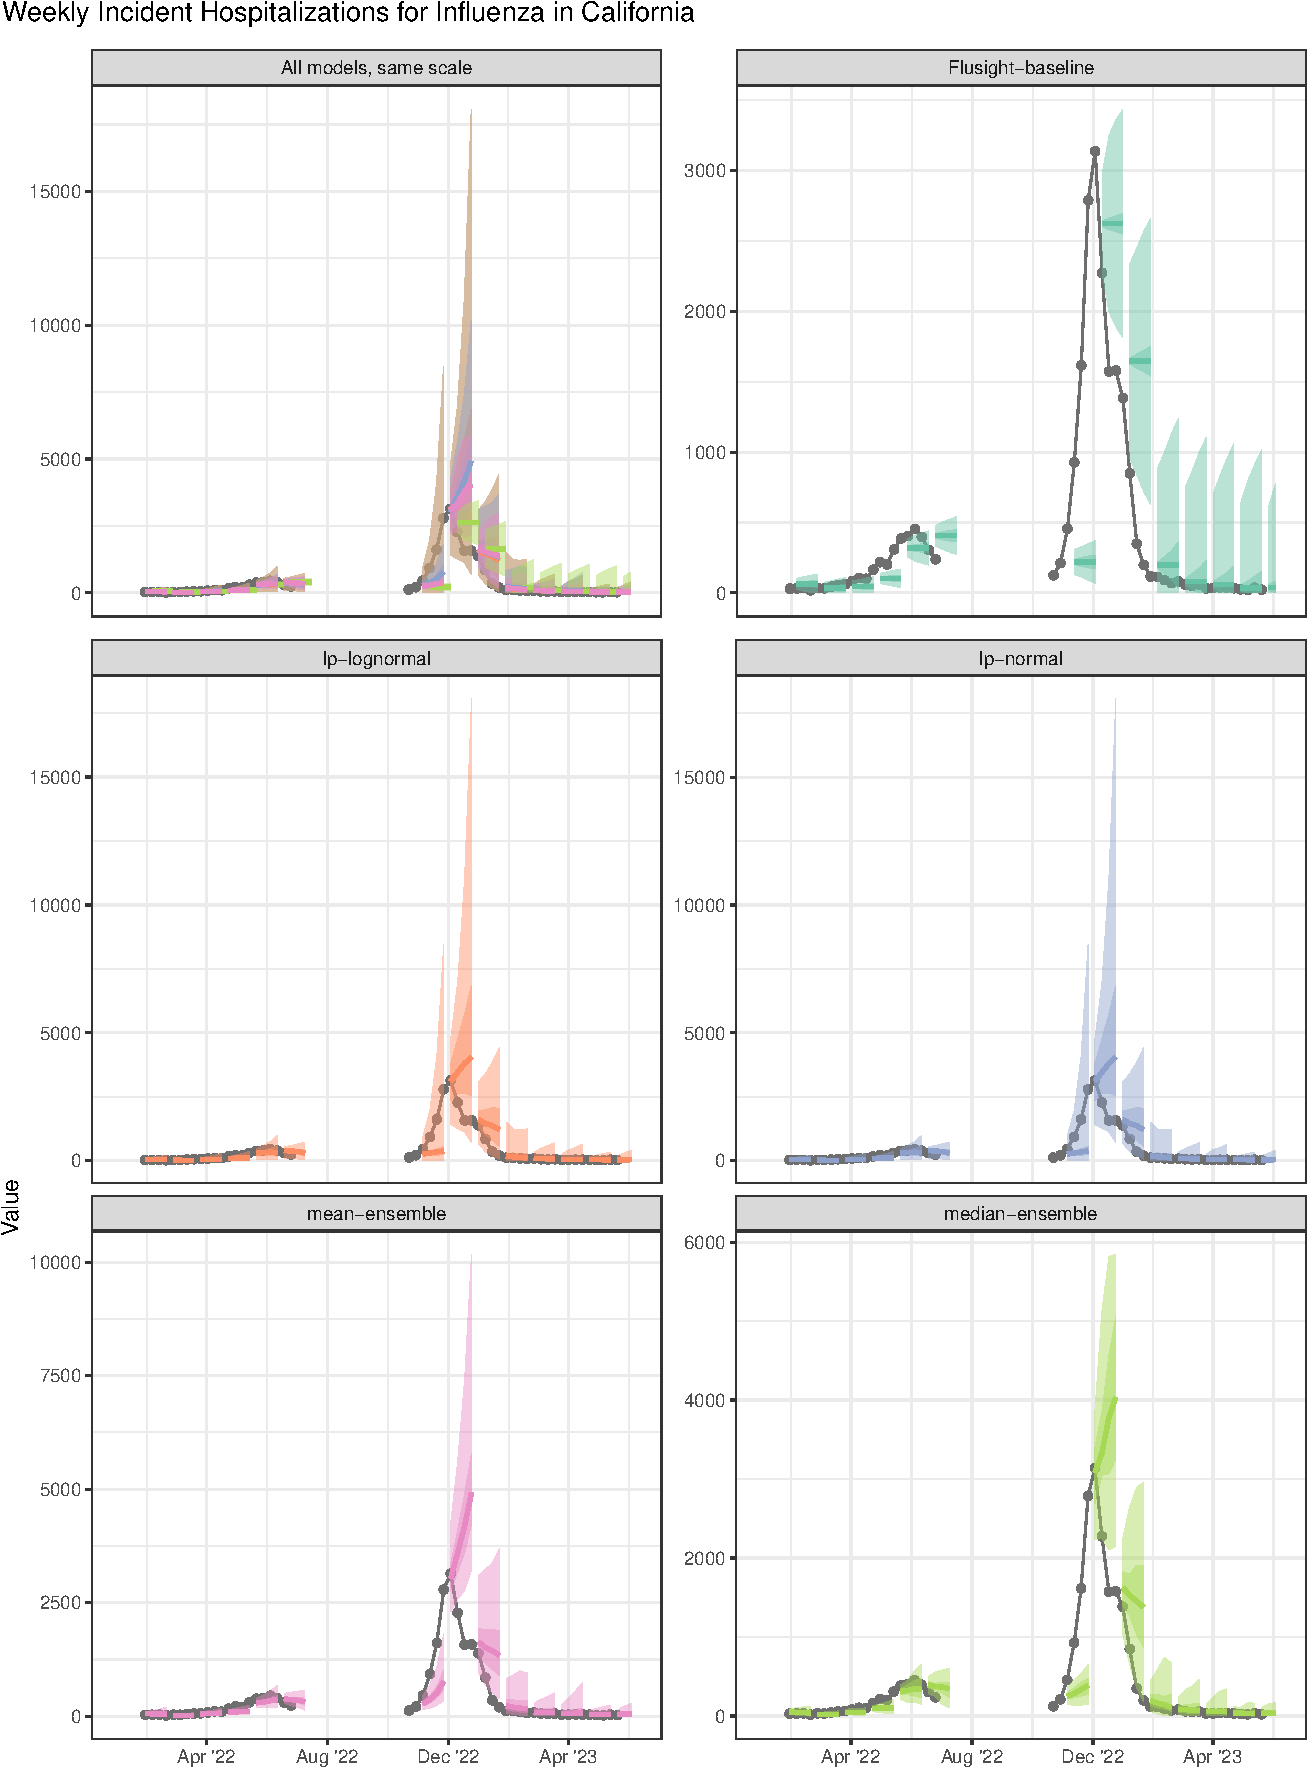
\includegraphics{hubEnsembles_manuscript_files/figure-pdf/fig-plot-forecasts-hubVis-1.pdf}

}

\caption{\label{fig-plot-forecasts-hubVis}One to four week ahead
forecasts for select dates plotted against target data for California.
The first panel shows all models on the same scale. All other panels
show forecasts for each individual model, with varying y-axis scales,
and their prediction accuracy as compared to observed influenza
hospitalizations.}

\end{figure}%

Averaging across all time points, the median model can be seen to have
the best scores for every metric. It outperforms the mean ensemble by a
similar amount for both MAE and WIS, particularly around local times of
change (see Figure~\ref{fig-mae-vs-forecast-date} and
Figure~\ref{fig-wis-vs-forecast-date}). The median ensemble also has
better coverage rates than the mean ensemble in the tails of the
distribution (95\% intervals, see
Figure~\ref{fig-cov95-vs-forecast-date}) and similar coverage in the
center (50\% intervals). The median model also outperforms the linear
pools for most weeks, with the greatest differences in scores being for
WIS and coverage rates (Figure~\ref{fig-wis-vs-forecast-date} and
Figure~\ref{fig-cov95-vs-forecast-date}). This seems to indicate that
the linear pools' estimates are usually too conservative, with their
wide intervals and higher-than-nominal coverage rates being penalized by
WIS. However, during the 2022-2023 season there are several localized
times when the linear pools showcased better one-week-ahead forecasts
than the median ensemble (Figure~\ref{fig-wis-vs-forecast-date}). These
localized instances are characterized by similar MAE values
(Figure~\ref{fig-wis-vs-forecast-date}) for the two methods and poor
median ensemble coverage rates
(Figure~\ref{fig-cov95-vs-forecast-date}). In these instances, the wide
intervals from the linear pools were useful in capturing the
eventually-observed hospitalizations, usually during times of rapid
change.

\begin{figure}

\centering{

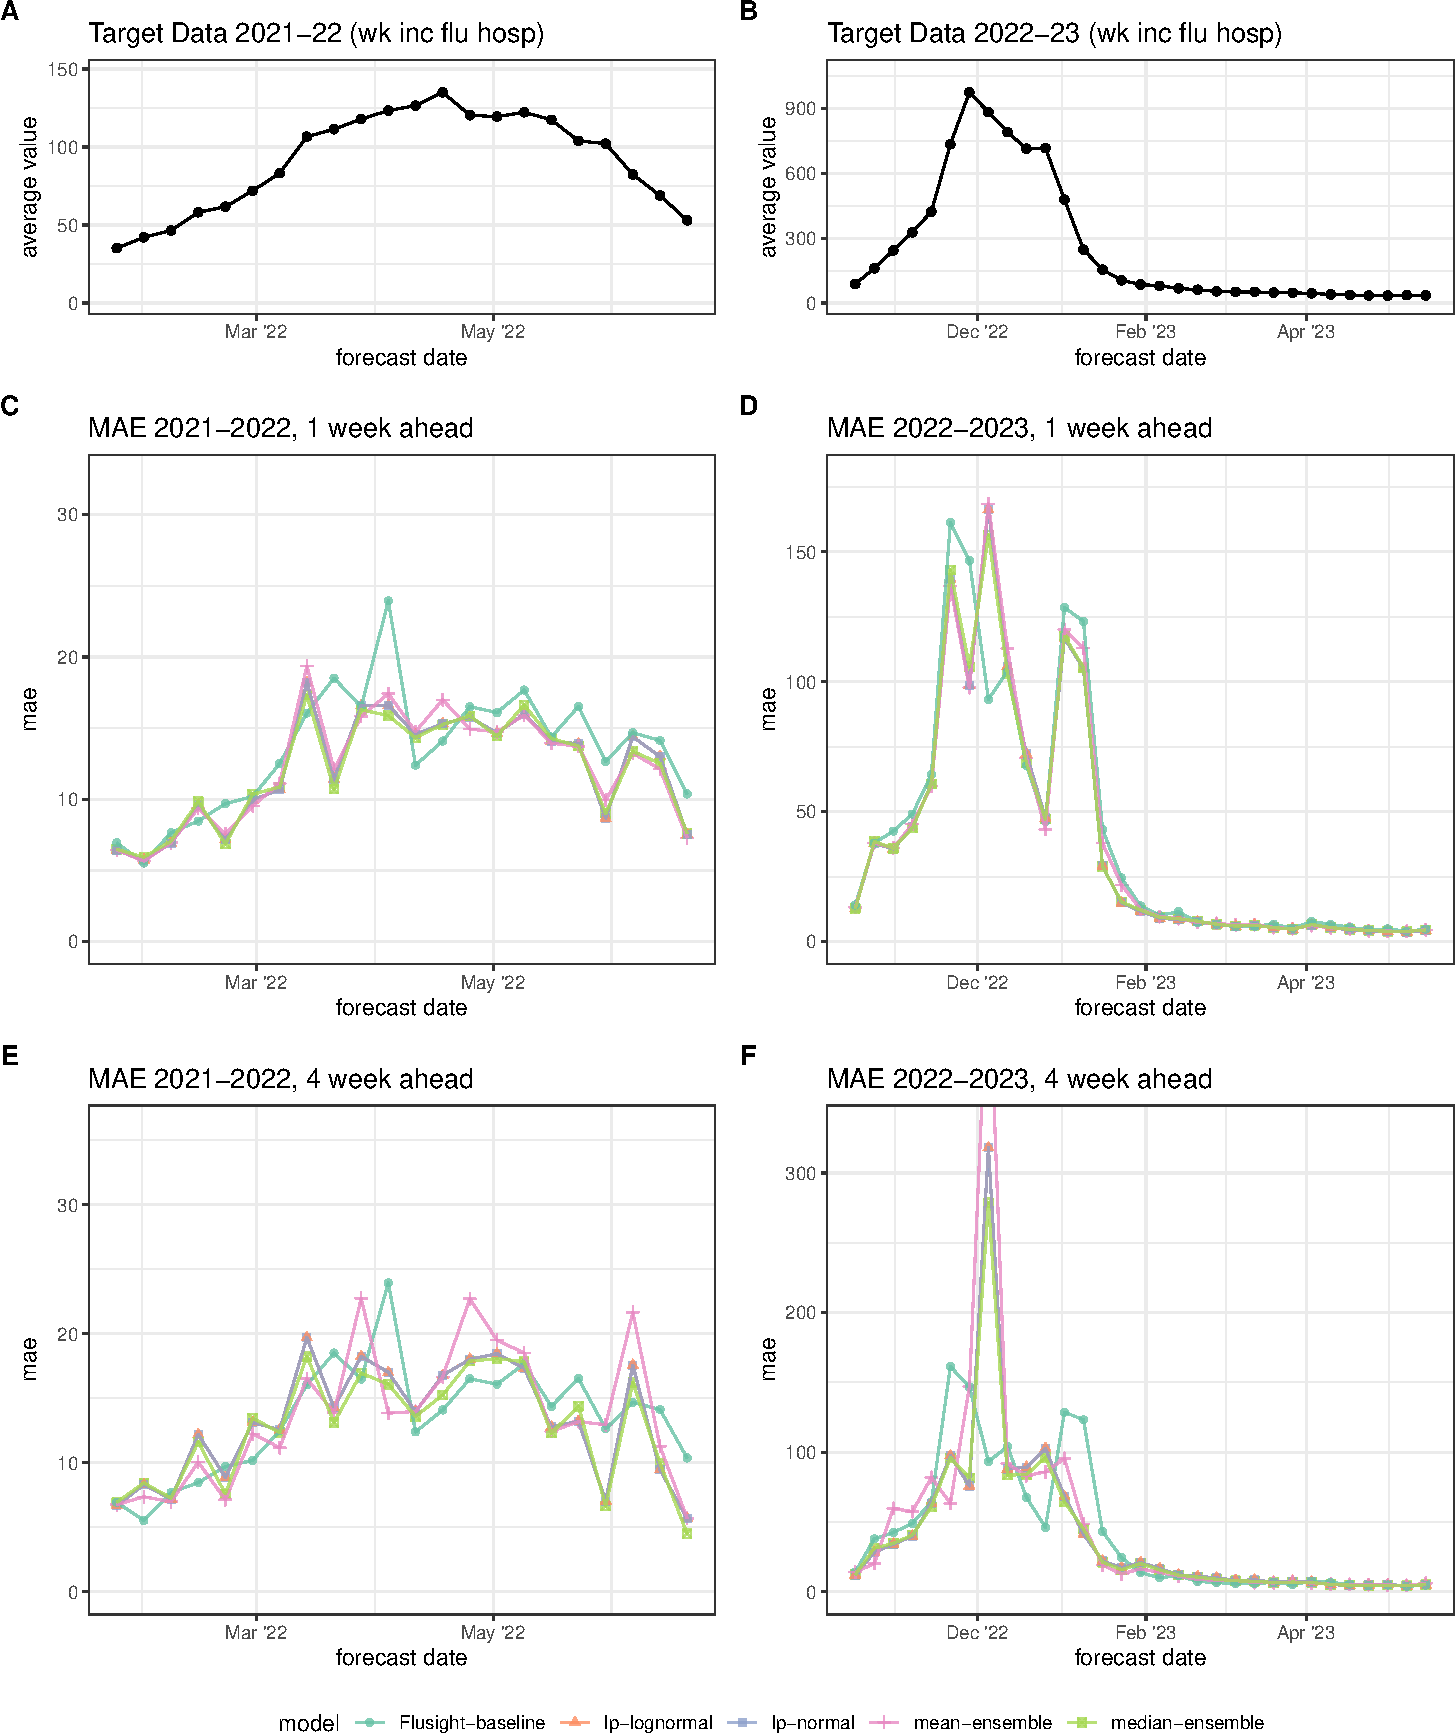
\includegraphics{hubEnsembles_manuscript_files/figure-pdf/fig-mae-vs-forecast-date-1.pdf}

}

\caption{\label{fig-mae-vs-forecast-date}Mean absolute error (MAE)
averaged across all locations. Average target data across all locations
for 2021-2022 (A) and 2022-2023 (B) seasons for reference. For each
season, average MAE is shown for 1-week (C-D) and 4-week ahead (E-F)
forecasts. Results are plotted for each ensemble model (colors) across
the entire season. Lower values indicate better performance.}

\end{figure}%

\begin{figure}

\centering{

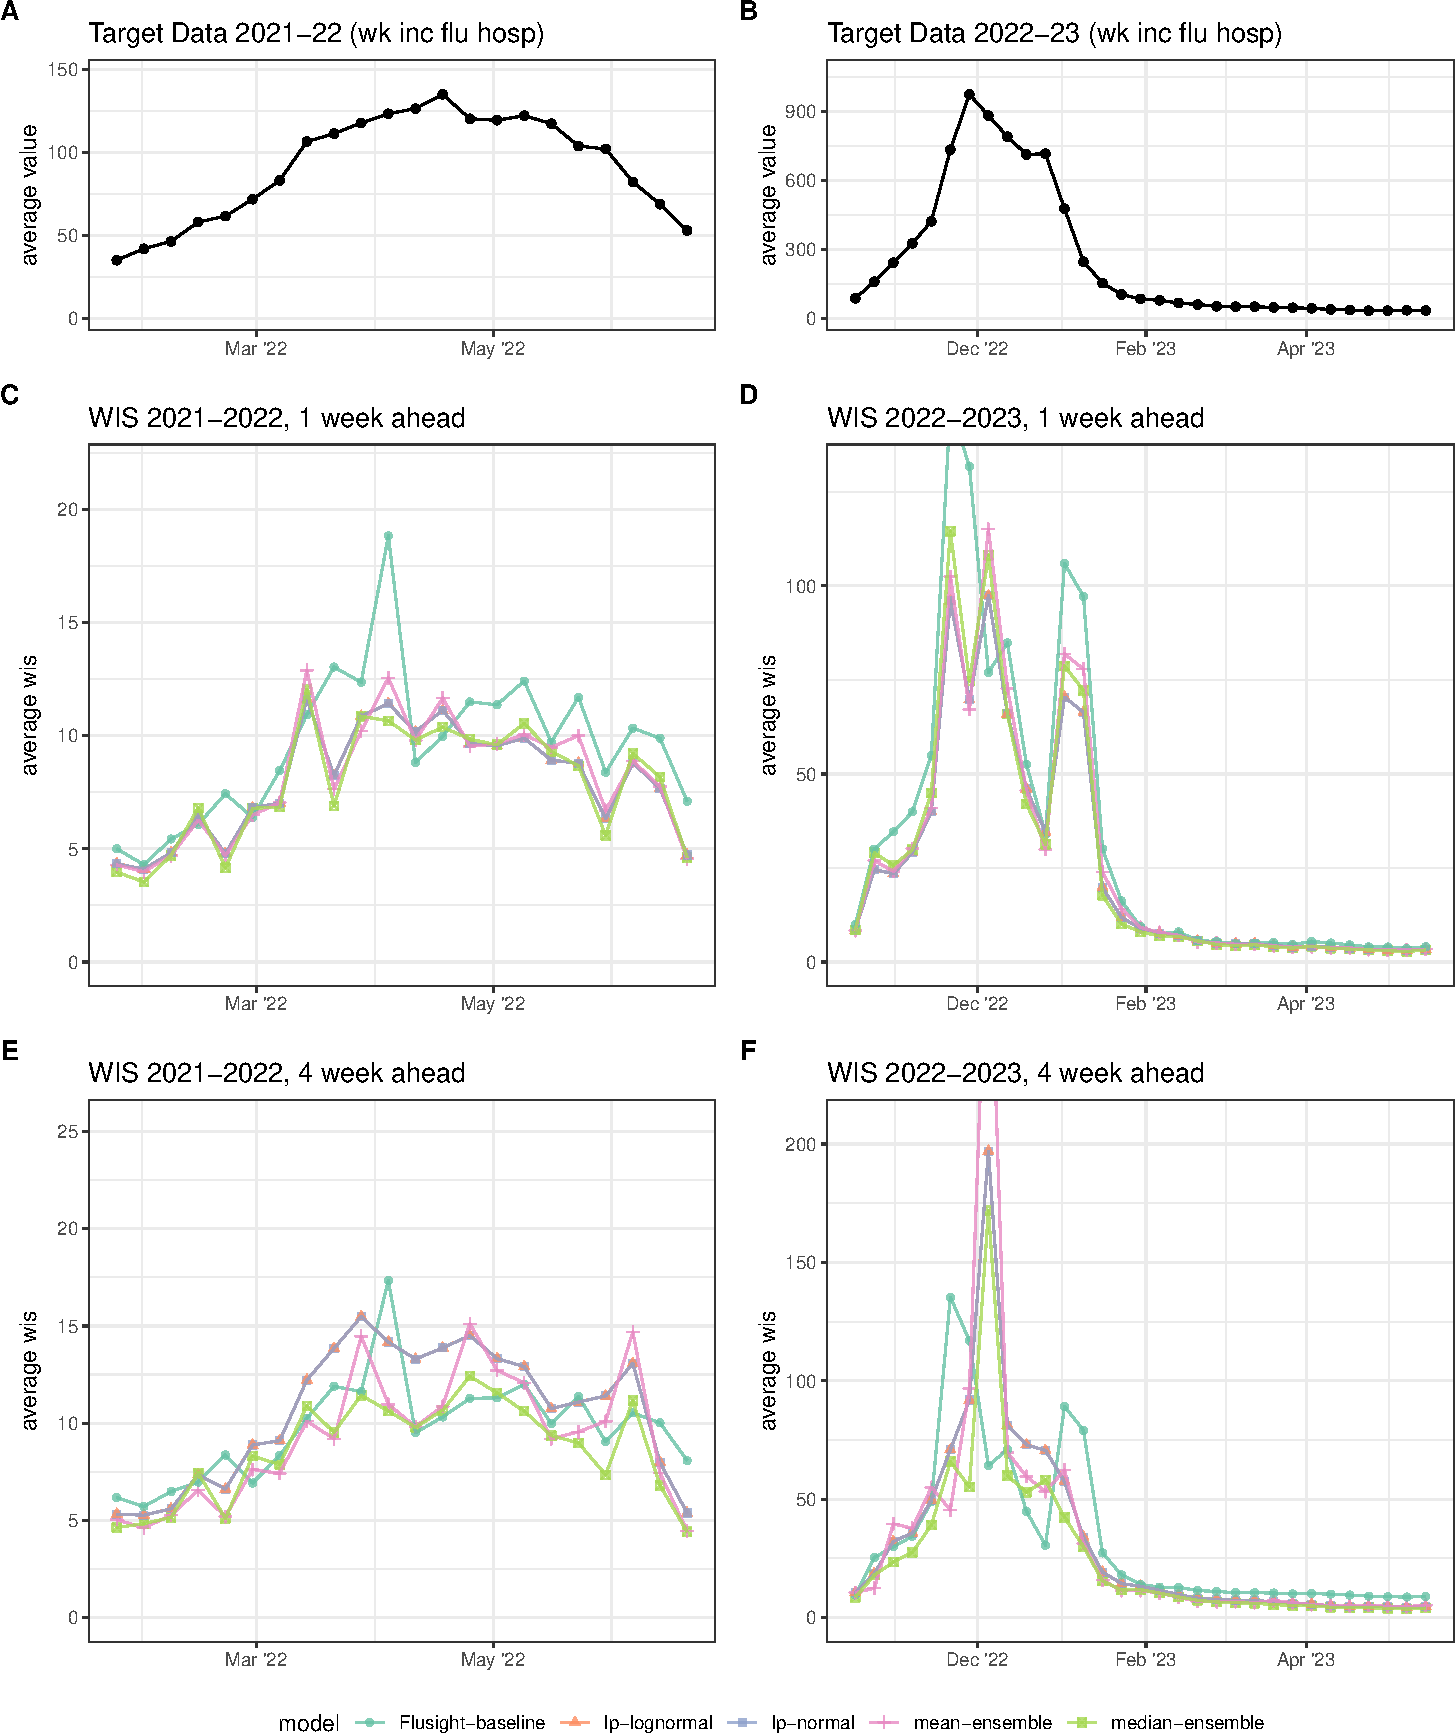
\includegraphics{hubEnsembles_manuscript_files/figure-pdf/fig-wis-vs-forecast-date-1.pdf}

}

\caption{\label{fig-wis-vs-forecast-date}Weighted interval score (WIS)
averaged across all locations. Average target data across all locations
for 2021-2022 (A) and 2022-2023 (B) seasons for reference. For each
season, average WIS is shown for 1-week (C-D) and 4-week ahead (E-F)
forecasts. Results are plotted for each ensemble model (colors) across
the entire season. Lower values indicate better performance.}

\end{figure}%

\begin{figure}

\centering{

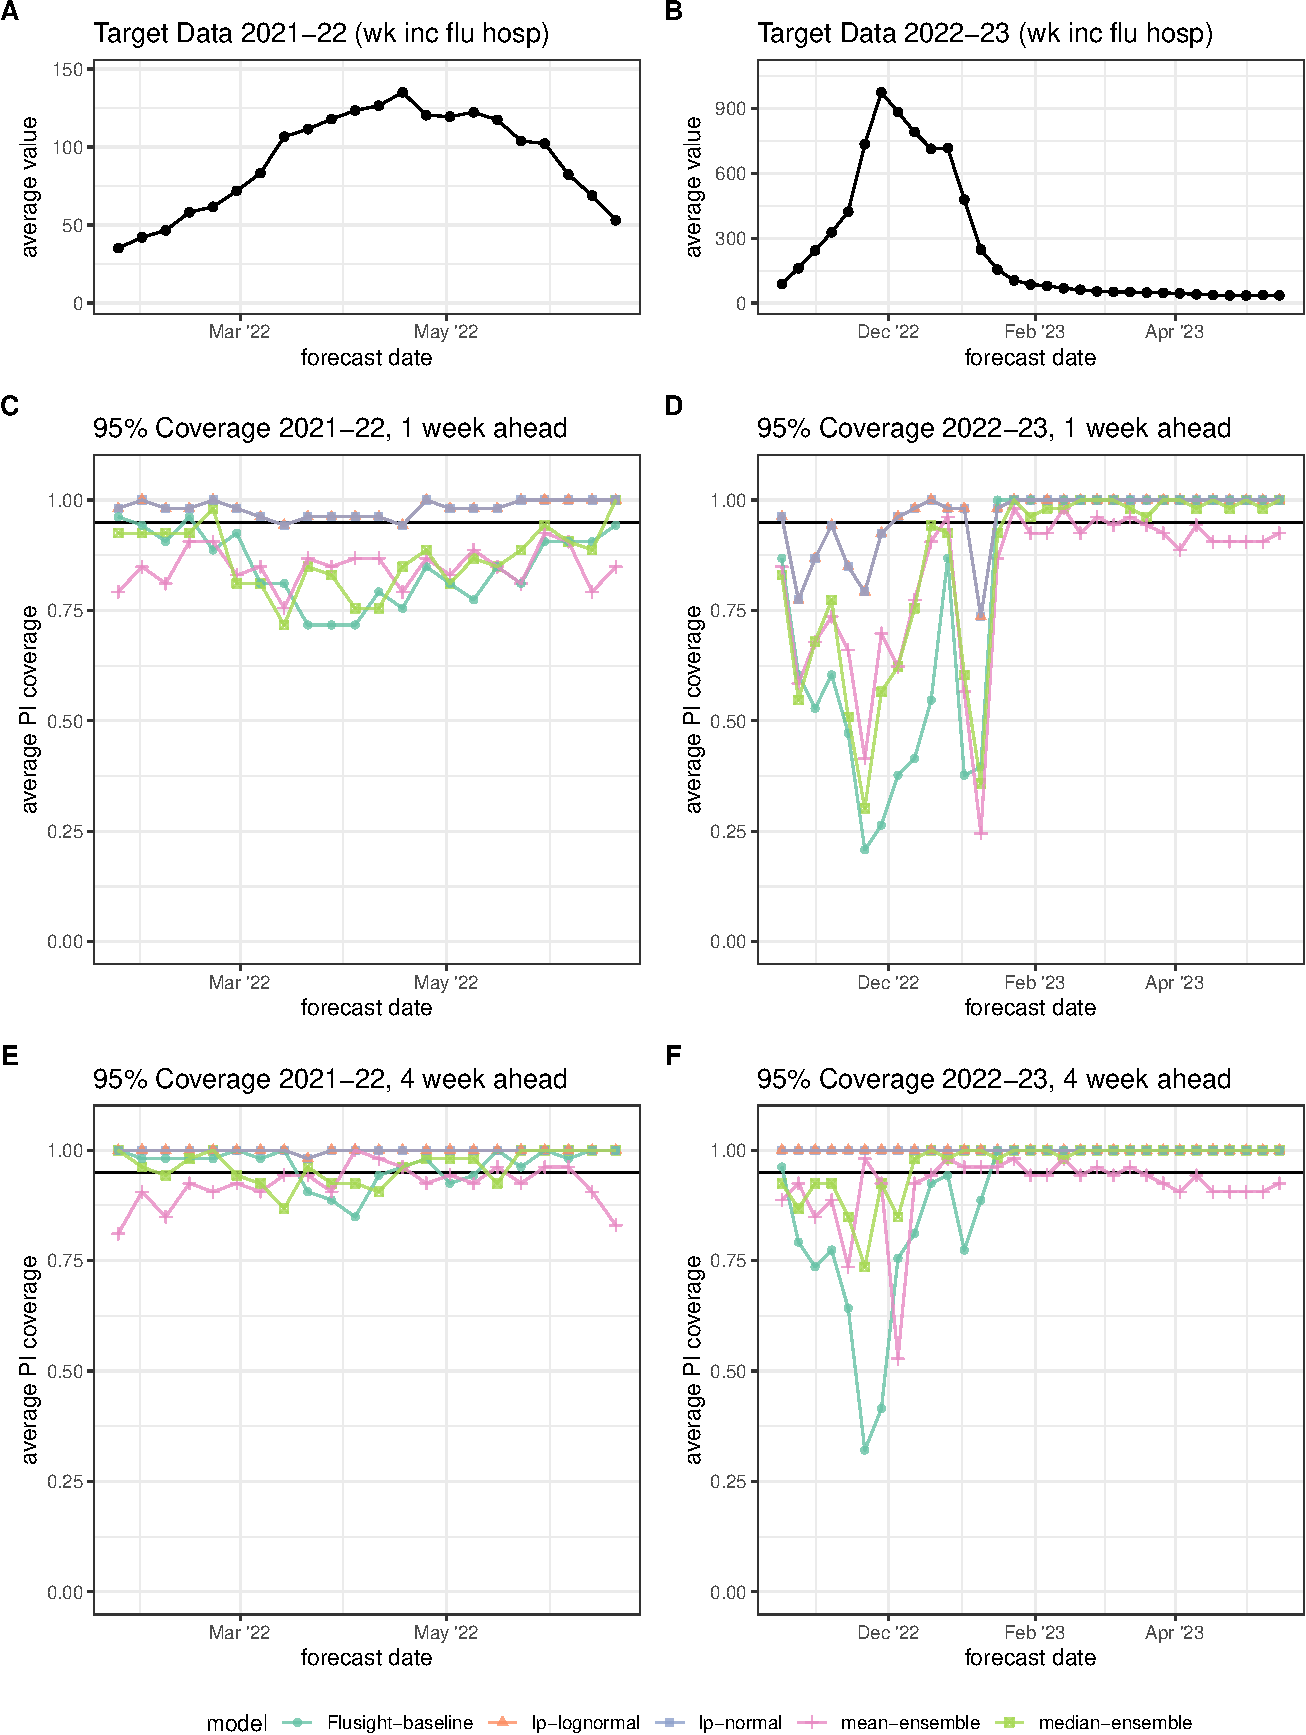
\includegraphics{hubEnsembles_manuscript_files/figure-pdf/fig-cov95-vs-forecast-date-1.pdf}

}

\caption{\label{fig-cov95-vs-forecast-date}95\% prediction interval (PI)
coverage averaged across all locations. Average target data across all
locations for 2021-2022 (A) and 2022-2023 (B) seasons for reference. For
each season, average coverage is shown for 1-week (C-D) and 4-week ahead
(E-F) forecasts. Results are plotted for each ensemble model (colors)
across the entire season. Ideal coverage of 95\% is shown (black
horizontal line); values closer to 95\%indicate better performance.}

\end{figure}%

In this analysis, all of the ensemble variations outperform the baseline
model; yet, different ensembling methods perform best under different
circumstances. While the quantile median has the best overall results
for WIS, MAE, 50\% PI coverage, and 95\% PI coverage, other models may
perform better from week-to-week for each metric. Around the 2022-2023
season's peak in early December, the remaining four models (including
the baseline) each have instances in which they achieve the lowest WIS,
like the linear pool ensembles for the one week ahead horizon over
several weeks of this period.

The choice of an appropriate ensemble aggregation method may depend on
the forecast target, the goal of forecasting, and the behavior of the
individual models contributing to an ensemble. One case may call for
prioritizing high coverage rates while another may prioritize accurate
point forecasts. The \texttt{simple\_ensemble()} and
\texttt{linear\_pool()} functions and the ability to specify component
model weights and an aggregation function for
\texttt{simple\_ensemble()} allow users to implement a variety of
ensemble methods.

\section{Summary and discussion}\label{sec-conclusions}

Ensembles of independent models are a powerful tool to generate more
accurate and more reliable predictions of future outcomes than a single
model alone. Here, we have demonstrated how to utilize
\pkg{hubEnsembles}, a simple and flexible framework to combine
individual model predictions into an ensemble.

The \pkg{hubEnsembles} package is situated within the larger hubverse
collection of open-source software and data tools to support
collaborative modeling exercises \citep{hubverse_docs}. Collaborative
hubs offer many benefits, including serving as a centralized entity to
guide and elicit predictions from multiple independent models
\citep{reich2022}. Given the increasing popularity of multi-model
ensembles and collaborative hubs, there is a clear need for generalized
data standards and software infrastructure to support these hubs. By
addressing this need, the hubverse suite of tools can reduce duplicative
efforts across existing hubs, support other communities engaged in
collaborative efforts, and enable the adoption of multi-model approaches
in new domains.

When using \pkg{hubEnsembles}, it is important to carefully choose an
ensemble method that is well suited for the situation. Although there
may not be a universal ``best'' method, matching the properties of a
given ensemble method with the features of the component models will
likely yield best results \citep{howerton2023}. Our case study on
seasonal influenza forecasts in the US demonstrates this point. The
quantile median ensemble performs best overall for a range of metrics,
including weighted interval score, mean absolute error, and prediction
interval coverage. Yet, the linear pool method, which generates an
ensemble with wider prediction intervals, demonstrates performance
advantages during periods of rapid change, when outlying component
forecasts are likely more important. Notably, all ensemble methods
outperform the baseline model. The performance improvements from
ensemble models motivate the use of a ``hub-based'' approach to
prediction for infectious diseases and in other fields.

Ongoing development of the \pkg{hubEnsembles} package and the larger
suite of hubverse tools will continue to support multi-model predictions
in new ways, including for example supporting additional types of
predictions, enabling scoring and evaluation of those predictions, and
allowing for cloud-based data storage. All such infrastructure will
ultimately provide a comprehensive suite of open-source software tools
for leveraging the power of collaborative hubs and multi-model
ensembles.

\section*{Acknowledgements}\label{acknowledgements}
\addcontentsline{toc}{section}{Acknowledgements}

The authors thank all members of the hubverse community; the broader
hubverse software infrastructure made this package possible. L.
Shandross, A. Krystalli, N. G. Reich, and E. L. Ray were supported by
the National Institutes of General Medical Sciences (R35GM119582) and
the US Centers for Disease Control and Prevention (U01IP001122 and
NU38FT000008). E. Howerton was supported by the Eberly College of
Science Barbara McClintock Science Achievement Graduate Scholarship in
Biology at the Pennsylvania State University. L. Contamin and H.
Hochheiser were supported by NIGMS grant U24GM132013. The content is
solely the responsibility of the authors and does not necessarily
represent the official views of NIGMS, the National Institutes of
Health, or CDC.

\section*{Consortium of Infectious Disease Modeling
Hubs}\label{consortium-of-infectious-disease-modeling-hubs}
\addcontentsline{toc}{section}{Consortium of Infectious Disease Modeling
Hubs}

Consortium of Infectious Disease Modeling Hubs authors include Alvaro J.
Castro Rivadeneira (University of Massachusetts Amherst), Lucie Contamin
(University of Pittsburgh), Sebastian Funk (London School of Hygiene \&
Tropical Medicine), Aaron Gerding (University of Massachusetts Amherst),
Hugo Gruson (data.org), Harry Hochheiser (University of Pittsburgh),
Emily Howerton (The Pennsylvania State University), Melissa Kerr
(University of Massachusetts Amherst), Anna Krystalli (R-RSE SMPC), Sara
L. Loo (Johns Hopkins University), Evan L. Ray (University of
Massachusetts Amherst), Nicholas G. Reich (University of Massachusetts
Amherst), Koji Sato (Johns Hopkins University), Li Shandross (University
of Massachusetts Amherst), Katharine Sherratt (London School of Hygene
and Tropical Medicine), Shaun Truelove (Johns Hopkins University),
Martha Zorn (University of Massachusetts Amherst)


\renewcommand\refname{References}
  \bibliography{references.bib}


\end{document}
